\documentclass[review,11pt]{elsarticle}
%\documentclass[preprint,review,12pt,authoryear]{elsarticle}
\usepackage{lineno,hyperref,ulem,todonotes}
\usepackage{rotating}
\usepackage{amsmath}
\modulolinenumbers[5]
%\usepackage{natbib}
\usepackage{tabularx,ragged2e,booktabs,caption}
\journal{Computational Geosciences}
\usepackage{multirow}
\usepackage{hhline}
\usepackage{placeins}

%%%%%%%%%%%%%%%%%%%%%%%
%% Elsevier bibliography styles
%%%%%%%%%%%%%%%%%%%%%%%
%% To change the style, put a % in front of the second line of the current style and
%% remove the % from the second line of the style you would like to use.
%%%%%%%%%%%%%%%%%%%%%%%

%% Numbered
\bibliographystyle{model1-num-names}

%% Numbered without titles
%\bibliographystyle{model1a-num-names}

%% Harvard
%\bibliographystyle{model2-names.bst}\biboptions{authoryear}

%% Vancouver numbered
%\usepackage{numcompress}\bibliographystyle{model3-num-names}

%% Vancouver name/year
%\usepackage{numcompress}\bibliographystyle{model4-names}\biboptions{authoryear}

%% APA style
%\bibliographystyle{model5-names}\biboptions{authoryear}

%% AMA style
%\usepackage{numcompress}\bibliographystyle{model6-num-names}

%% `Elsevier LaTeX' style
%\bibliographystyle{elsarticle-num}
%%%%%%%%%%%%%%%%%%%%%%%

\begin{document}

\begin{frontmatter}

%\title{Simulation Study of a Novel Subgrid Model for Microtopography Effect on Surface Flow}
\title{Modeling Microtopographic Effects in Watershed-scale Integrated Surface/Subsurface Models}
%\author[ornl]{Ahmad Jan \corref{cor}} \author[lanl1]{Ethan T. Coon} \author[ornl]{Scott L. Painter} \author[lanl2]{Rao Garimella} \author[lanl2]{J. David Moulton}

%\address[ornl]{Climate Change Science Institute and Environmental Sciences Division, Oak Ridge National Laboratory, Oak Ridge, Tennessee, USA\fnref{copyrightnotice}} 
%\address[lanl1]{Computational Earth Sciences Group, Earth and Environmental Sciences Division, Los Alamos National Laboratory, Los Alamos, New Mexico, USA} 
%\address[lanl2]{Applied Mathematics and Plasma Physics Group, Theoretical Division, Los Alamos National Laboratory, Los Alamos, New Mexico, USA} 


%\cortext[cor]{Corresponding Author: Ahmad Jan; Email: jana@ornl.gov; Phone: (865) 576-8175.}


\begin{abstract}
Permafrost-affected regions in the Arctic manifest a patterned ground, mainly characterized by ice-wedge polygons. The role of patterned polygonal ground and associated small-scale microtopography (spatial heterogeneities at a scale smaller than the size of polygons) in controlling surface/subsurface thermal hydrology is critical but conceptually well-understood. Accurate representation of microtopographic influences on flow requires fine-scale simulations, and simulating standalone fine-scale surface hydrology is feasible with modern computing tools. However, highly resolved integrated surface/subsurface thermal hydrology simulations are not tractable at watershed scale and requires proper modeling. To capture the effects of microtopographic features (such as depressions, obstructions) in coarsened model, we present a subgrid model parameterized by small-scale spatial heterogeneities.  The subgrid model alters the water storage and flow terms in the existing governing equations. We demonstrate how a few parameters extracted from the available fine-scale information can be utilized to account for microtopographic effects in coarsened watershed-scale integrated models.
Simulations were carried out and numerical results of the subgrid model were compared both to those generated with no subgrid model and to fine-scale results of seven ice-wedge polygons. Our findings confirm that the subgrid model improves the shape of hydrographs and total water content in the system, and that the results are very close to the corresponding fine-scale simulations. Watershed-scale fully integrated surface/subsurface simulations with the subgrid model yield expected results. For three scenarios based on the spatial distribution of the subgrid parameters, we observe significant difference in the hydrology (increased infiltration, reduced runoff), however our results show that the subgrid model has less effect on the thermal conditions and active layer thickness.  
\end{abstract}

\begin{keyword}
Subgrid model \sep Microtopography  \sep  Polygonal tundra \sep  Watershed \sep Integrated Surface/Subsurface simulations
\end{keyword}


\end{frontmatter}

\linenumbers

\FloatBarrier
\section{Introduction}\label{introduction}
To better understand the interactions between surface/subsurface, surface runoff and discharge rate, it is important to gain insight into the role of
heterogeneous spatial structure of the ground surface.
It is well understood that spatial heterogeneities in the surface microtopography (unevenness at small scale) serve a critical role in surface water retention, surface/subsurface interactions, delay runoff, and thereby significantly affects the shape of hydrographs~\cite{toth1962theory,dunne1991effects,holden2005peatland, kvaerner2008generation, huang2009influences, andresen2015disappearing}. In general, an accurate flow representation is achieved at fine-scale (a scale of centimeters) and fortunately with the availability of sophisticated simulation tools, standalone highly resolved surface-flow simulations are easily tractable. However, fully integrated surface/subsurface thermal hydrology simulations with highly resolved computational grid are not tractable at watershed scale. Frei et. al.~(\citeyear{frei2010effects}) in their work reported a computational time of two months to simulate a year-long modeling scenario at a plot-scale (10-20m), which is a huge computational cost. However, accurate representation of runoff (both qualitatively and quantitively) at watershed- or hillslope-scale simulations is accomplished when micro-scale effects are incorporated in the hydrological models~\cite{bronstert1997modelling,nakayama2006simulation}. Thus, if the microtopographic effects are ignored in the integrated models, the processes representing flow will not be completely accurate. 
The idea to incorporate fine-scale flow behavior in watershed-scale integrated models without: (i) significant computational cost, and (ii) high-resolved grid, motivates the use of subgrid representation in coarsened models. A subgrid model is build on the information gained from highly resolved surface topographic data: the depressions and obstructions. Depressions are disconnected low points in the topography (surface pits) that retain water that is available only for infiltration or/and evaporation. Obstructions are objects exit above the depressions that interrupt and slow the flow, but do not completely block it. 

Fully coupled surface/subsurface three-dimensional simulations in a complex hydrological environment at larger spatiotemporal scales is a challenging task even if coarsened models are considered~\cite{frei2010effects}. Further significant challenges arise when simulating permafrost dynamics because a more complex set of governing equations needs to be solved to accurately represent all the relevant processes~\cite{painter2013modeling,jan2017}. We have recently developed a mixed-dimensional model to efficiently simulate surface/subsurface thermal hydrology of permafrost-affected landscapes at watershed scales; reported in~\cite{jan2017}. In this modeling approach, the subsurface is discretized as independent columns and coupled through a surface flow system; more details are provided in the subsequent sections. Here we intend to apply the subgrid parametrization to the lateral flow part only (two-dimensional surface system) in the mixed-dimensional modeling approach. This is one aspect of incorporating the microtopographic effects in watershed-scale integrated models, however, in general, both the surface and subsurface require a subgrid model. 
In this work, we are testing a hypothesis that the effects of microtopography can be captured in coarsened models through the use of a subgrid model. We evaluate one possible form of that model, and explore how parameters can be deduced from the available information.

 %--------------------------
Here we use polygonal tundra as an example. Tundra landscapes exhibit patterned polygonal ground (illustrated in Figure~\ref{tundra-sitesA-B}) developed by repeated freezing and thawing of ground soil. Thawing ice-wedge polygons results in a complex mosaic of topographic patterns and lead to spatial heterogeneities both at and below the scale of the size of polygon. We call spatial scale variability in the topography at and below the scale of the size of polygon as macro- and micro-topography, respectively. Small scale features of the polygonal landscapes can have regional impacts on hydrology, active-layer thickness and permafrost degradation. Thus simulating permafrost soils at a scale of macrotopography (or larger) without taking small-scale information into account could lead to inaccurate estimate of carbon release and energy balance etc. under warming trends in the Arctic landscapes; for example see~\cite{liljedahl2016pan,lu2012modeling,andresen2015disappearing,holden2005peatland}. More details are provided in section~\ref{field-site}.
\begin{figure}[!h]
\centering
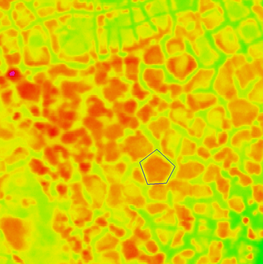
\includegraphics[width=9.5cm, height=8cm]{./figures/DEM_Area_B-HCP.png} \\
\hspace*{0.8cm}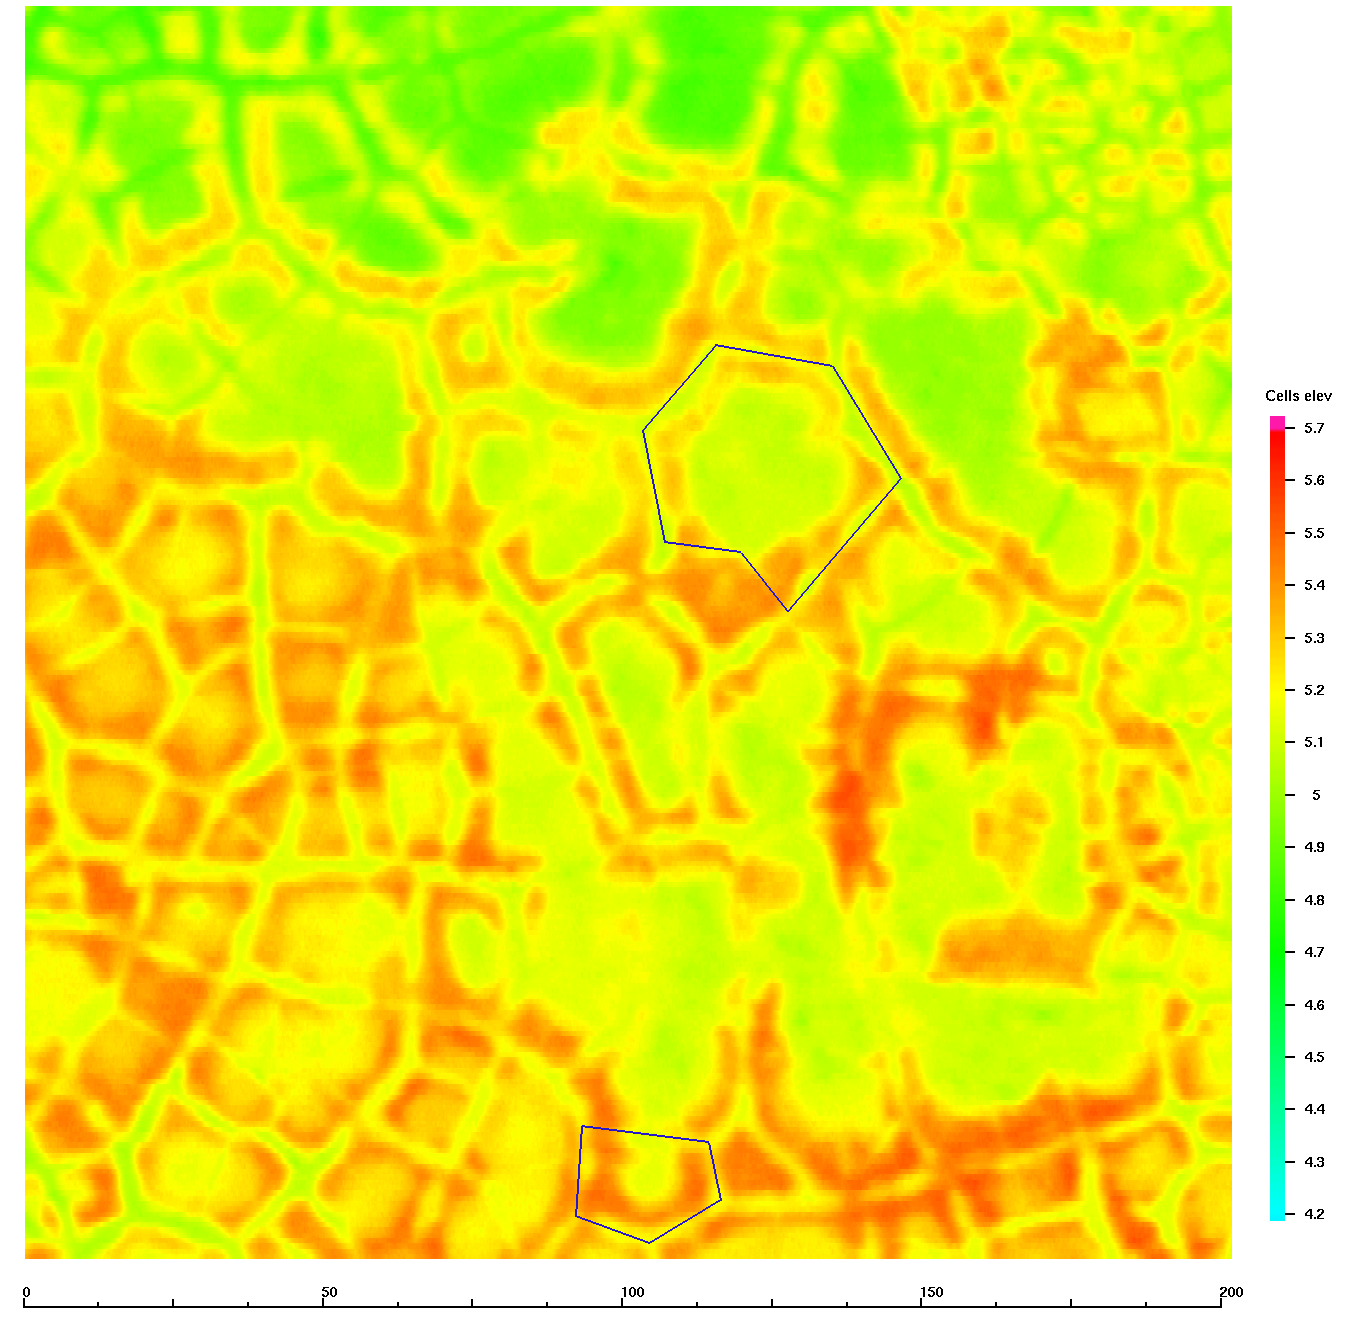
\includegraphics[width=10.8cm, height=8cm]{./figures/DEM_Area_A-LCP.png}
\caption{An illustration of a patterned polygonal tundra landscape characterized by high-centered (top) and low-centered (bottom) polygons, located at NGEE-Arctic field sites A and B within Barrow Environmental Observatory (BEO) near Alaska, see Figure~\ref{ngee-arctic-fieldsites}.}
\label{tundra-sitesA-B}
\end{figure}

Pertinent to the literature, integrated suface/subsurface modeling has received considerable attention from researchers across the world; see, for example,~\cite{painter2013modeling,kurylyk2014climate,spainter2016integrated} and references therein. Here we focus only on the subgrid modeling approach. Though the concept of microtopographic features and their implications on the flow and discharge is not new, but has not been fully addressed and understood from modeling perspective. 
% -----------------------------------------------------------------------------------------------------------------------------------------------------------------------------------
In the mid-1950s, the significance of the surface microtopographic features were described in~\cite{stammers1956effect}. Panday and Huyakorn (\citeyear{panday2004fully}) presented an integrated surface/subsurface flow model with subgrid representation through the surface depressions and obstructions by modifying the overland flow governing equation. A one-dimensional simulations to study the effects of spatially varying surface roughness on flow hydrographs is presented in~\cite{huang2009influences}. In a numerical experiment at a scale of a few meters, Frei et al.~(\citeyear{frei2012surface}) highlighted that surface microtopography in wetlands can lead to the formation of biogeochemical hot spots. A spatially varying rill/depression storage concept to account for microtopographic effects in a plot scale simulations for integrated surface/surface flow is presented in~\cite{frei2014representing}.
%-----------------------------------------------------------------------------------------------------------------------------------------------------------------------------------------------

The rest of the paper is organized as follows. Section \ref{field-site} introduces the Arctic patterned polygonal ground. Section~\ref{subgridmodel} presents the derivation of the governing equations of the subgrid model. A short description, for a quick reference, of the Advanced Terrestrial Simulator (ATS) and the Arcos multiphysics management framework, within which we implemented our subgrid model, is presented in Section~\ref{ATS}. In Section~\ref{numerical-tests} we compare the numerical results of our subgrid model with no subgrid model and fine-scale results to illustrate the accuracy of our subgrid model for capturing fine-scale microtopographic features. Finally, in Section~\ref{conclusion}, we offer closing remarks and future research inline with thaw-induced subsidence.


\section{Field Site: Arctic Patterned Polygonal Ground}\label{field-site}
A large amount of frozen organic carbon is stored in permafrost-affected soils of the Northern Hemisphere~\cite{schuur2015climate,bg-11-6573-2014}. The ground in the Arctic regions is temperature-sensitive and under potential risk of carbon release to the atmosphere in a changing climate~\cite{hinzman2005evidence}.
Arctic landscapes are dominated by polygonal patterned (interconnected polygons) ground. The formation of polygonal landscapes in permafrost-affected regions is a consequence of recurring cracks-compression process over hundreds of thousands of years. During winter, vertical fractures are formed due to ground contraction, the water from the snowmelt in the following summer penetrates those cracks and refreezes. In the following winter, the reexpansion of the ice in the cracks compresses the soil horizontally. The recurring crack-compression process over long period of time develops wedges of ice and finally a polygonal landscape is formed~\cite{lachenbruch1962mechanics,greene1963contraction,mackay1990some,mackay2004thermally}. Figure~\ref{ngee-arctic-fieldsites} displays a polygonal tundra, a field site of the U.S. Department of Energy's Next Generation Ecosystem Experiments (NGEE) Arctic project located within the Barrow Environmental Observatory (BEO)~\cite{kumar2016modeling}.
\begin{figure}[!h]
\centering
 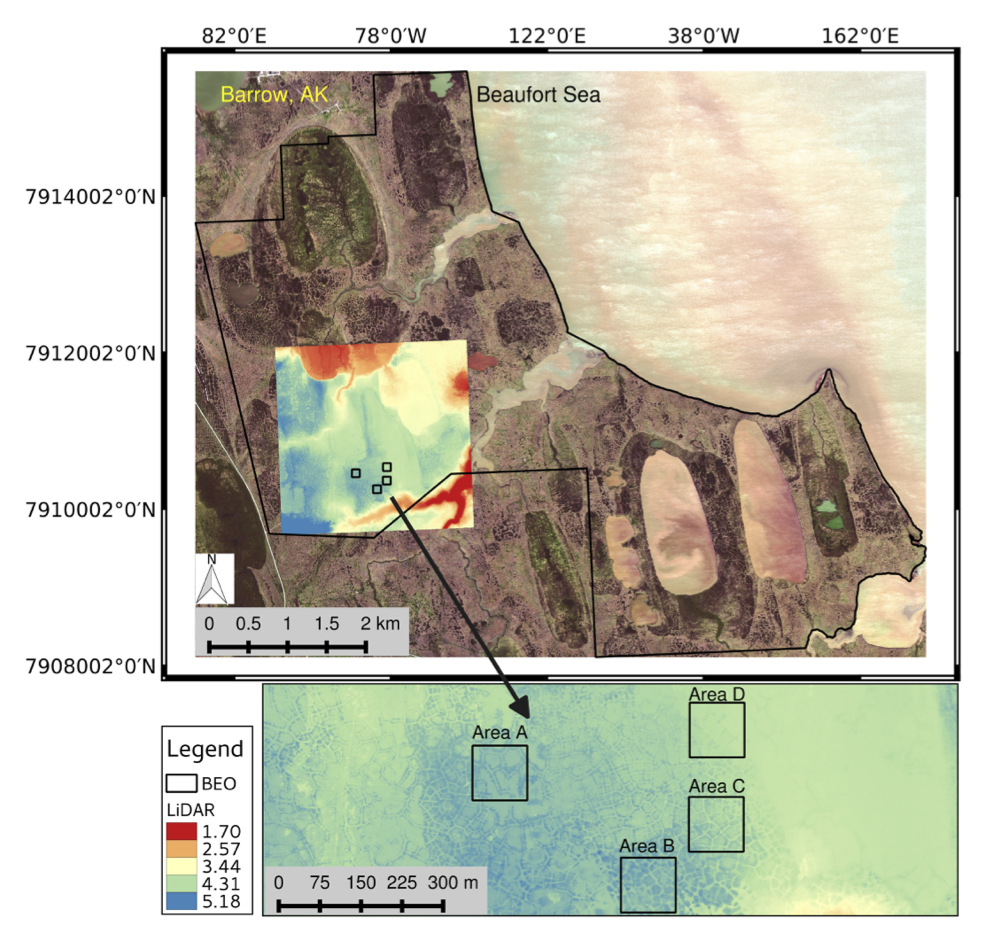
\includegraphics[width=14cm, height=17cm]{./figures/ngee-arctic-fieldsites.png}
\caption{NGEE-Arctic field sites at BEO~\cite{kumar2016modeling}.}
\label{ngee-arctic-fieldsites}
\end{figure}
Several types of polygons are formed due to permafrost degradation. Typically, the polygons are classified as low-centered polygon (LCP) and high-centered polygon (HCP) based on surface microtopography. The LCP has a raised rim and central depression, thereby holds ponded water in the center during the summer that can only be available for infiltration and evaporation. The HCP has elevated center that slopes downward to trough and enhances runoff, thus the center may remain mostly dry. 
Thawing of ice-wedges causes the raised rims of LCP to subside that leads to the formation of HCP~\cite{jorgenson2006abrupt}. The loss of depression storage in the LCP has the ability to connect the disconnected troughs, thus transforms a poorly drained tundra to a well-established drainage network. Those changes will potentially alter the entire ecosystem and will bring substantial hydrological changes (e.g., surface/subsurface interactions, distribution of surface water, discharge rate etc.)~\cite{liljedahl2016pan, hinzman2005evidence,rowland2010arctic,liljedahl2012ice}.



\section{Surface Flow Model}\label{surf-flow-system}
This section describes diffusion wave equation for surface flow representation. In this work, we will be referring to three types of models as follow:
\begin{description}\itemsep0pt \parskip0pt
\item I. (Fine-scale model) Diffusion wave equation with high-resolved mesh (centimeter-scale grid spacing).
\item II. (No subgrid model) Diffusion wave equation with coarsened mesh (meter-scale grid spacing).
\item III. (Subgrid model) Modified diffusion wave equation (derived in subsection~\ref{subgridmodel}) with coarsened mesh (meter-scale grid spacing).
\end{description}
In Models II and II, the grid is a planer surface with a specified slope, and corners are consistent with the corners of the fine-scale mesh.
\subsection{Diffusion Wave Equation}
Diffusion wave equation for surface flow representation is given by,
\begin{equation}\label{diffwaveeq}
\frac{\partial \delta}{\partial t} + \nabla \cdot (\delta V)= q_\text{rp} + \Gamma_\text{ex}.
\end{equation}
Here $\delta$ represents ponded depth [L], $q_\text{rp}$ is rain precipitation rate [L$^3$/(L$^2 \cdot$ T)], $\Gamma_\text{ex}$ is water exchange between surface and subsurface systems [L$^3$/(L$^2 \cdot$ T)], $t$ is time [T], and $V$ denotes surface flow velocity given by,
\begin{equation}
V = - \frac{\delta^{2/3}}{n_\text{man} (\| \nabla Z\| +\epsilon)^{1/2}} \nabla(Z + \delta),
\end{equation}
where $n_\text{man}$ is Manning's coefficient [L$^{-1/3} \cdot$ T)], $Z$ is surface elevation [L], and $\epsilon >0$ is a regularization parameter used to avoid zero bed slope. More details about the models implemented in ATS can be found here~\cite{spainter2016integrated}. 
%Units are provided in Table~\ref{table1}.
%\begin{center}
%\begin{table}[htbp]
%\caption{Physical quantities with units}
%\begin{tabular}{| l | l |}
%\hline
%Physical quantities & SI units \\ \hline
%Ponded depth $(\delta)$ & m \\
%Elevation $(Z)$ & m \\
%Rain precipitation rate ($q_\text{rp}$) & m$^3/($m$^2$ s) \\
%Exchange term $(\Gamma_\text{ex})$& m$^3/($m$^2$ s) \\
%Manning's coefficient ($n_\text{man}) $ & m$^{-1/3}$ s \\
%Time ($t$) & s \\
%\hline
%\end{tabular}
%\label{table1}
%\end{table}
%\end{center}
\subsection{Subgrid Model}\label{subgridmodel}
Subgrid model incorporates depressions and obstructions in coarsened models to capture microtopgraphic effects on flow. It requires to alter accumulation term and flow law in the diffusion wave equation given by Equation~\ref{diffwaveeq}.
For example, the ponded depth $(\delta)$ in the accumulation term is typically replaced with a volumetric depth, the ponded depth that would occur if the surface were flat. A modified flow velocity is introduced to account for depressions and obstructions. A modified version of the diffusion wave equation with subgrid representation can be expressed as
\begin{equation}\label{diffwaveeq}
\frac{\partial \Phi (\delta)}{\partial t} + \nabla \cdot (\delta U)= q_\text{rp} + \Gamma_\text{ex}.
\end{equation}
Here the volumetric depth $\Phi (\delta)$ [L] and modified flow velocity $U$ are given by Equations~\ref{volumetric-depth2} and~\ref{modified-velocity}, respectively, and discussed in the subsequent subsections.
\subsubsection{Derivation of Volumetric Depth}
The volumetric head may be calculated on geometric arguments. Specifically, if the microtopographic elevation field on an ice-wedge polygon (IWP) is $Z_*(x,y)$, the the volumetric depth is
\begin{equation}\label{volumetric-depth1}
\Phi (\delta) = \frac{1}{A} \iint \left( \delta + Z_0 - Z_*(x,y) \right ) H \left( \delta + Z_0 - Z_*(x,y) \right ) dx dy.
\end{equation}
Where the integration is over the surface of the IWP, $A$ is the area of the IWP, $Z_0$ is the minimum elevation in the IWP, and $H$ is the Heaviside function. This could be computed from the microtopography and stored as a lookup table. Or, we could employ a simpler parameterization. To that end, we consider parameterizing the microtopography with two parameters: (1) the elevation range spanned by the subgrid microtopography $\delta_\text{max}$, and (2) the specific excluded volume $\delta_\text{ex}$, which is the soil volume per unit bulk area. Then, we approximate the volumetric depth as
\begin{equation}\label{volumetric-depth2}
\Phi (\delta) =
\begin{cases} (2 \delta_\text{max} - 3 \delta_\text{ex}) \left(\frac{\delta}{\delta_\text{max}} \right )^2 + (2 \delta_\text{ex} -  \delta_\text{max}) \left(\frac{\delta}{\delta_\text{max}} \right )^3 & \text{if} \hskip 0.1in 0 \leq \delta \leq \delta_\text{max}, \\
\delta - \delta_\text{ex} & \text{if} \hskip .1in \delta > \delta_\text{max}.
\end{cases}
\end{equation}
%The IWP shown in Fig~\ref{3Dpolygon40} was used to evaluate the parameterization Equation~\ref{volumetric-depth2}. 
The volumetric depth calculated from the approximation (Equation~\ref{volumetric-depth2}) is compared (curve) with the direct calculation (Equation~\ref{volumetric-depth1} (dots) ) for four ice-wedge polygon in Figure~\ref{volumetric-depth-fig1} and representative of other polygons. Also, shown is the volumetric depth in the absence of microtopography, which is linear with slope unity. Equation~\ref{volumetric-depth1} is a very good approximation.
\subsubsection{Modified Flow law}
Microtopographic effects on the flow law are not as straightforward to incorporate as the volumetric head $\Phi(\delta)$. In particular, we should make the distinction between depressions and obstractions~\cite{panday2004fully}. Depressions are disconnected low points in the topography. The ponded depth must rise above the level of those depressions before any flow can happen. Obstructions exist above the depressions and interrupt and slow the flow, but do not block it completely.
To model the effects of obstructions and depressions, we propose the following modification to the flow law
\begin{equation}\label{modified-velocity}
U = - \Theta(\delta) \frac{(\delta - \delta_\text{d})^{2/3}}{n_\text{man} (\| \nabla Z \| +\epsilon)^{1/2}}
\end{equation}
where $\delta_\text{d}$ is the depression depth [L], and $\Theta(\delta) \in [0,1]$ is a fractional conductance which accounts for flow reduction by obstructions.
%\begin{figure}
%\centering
%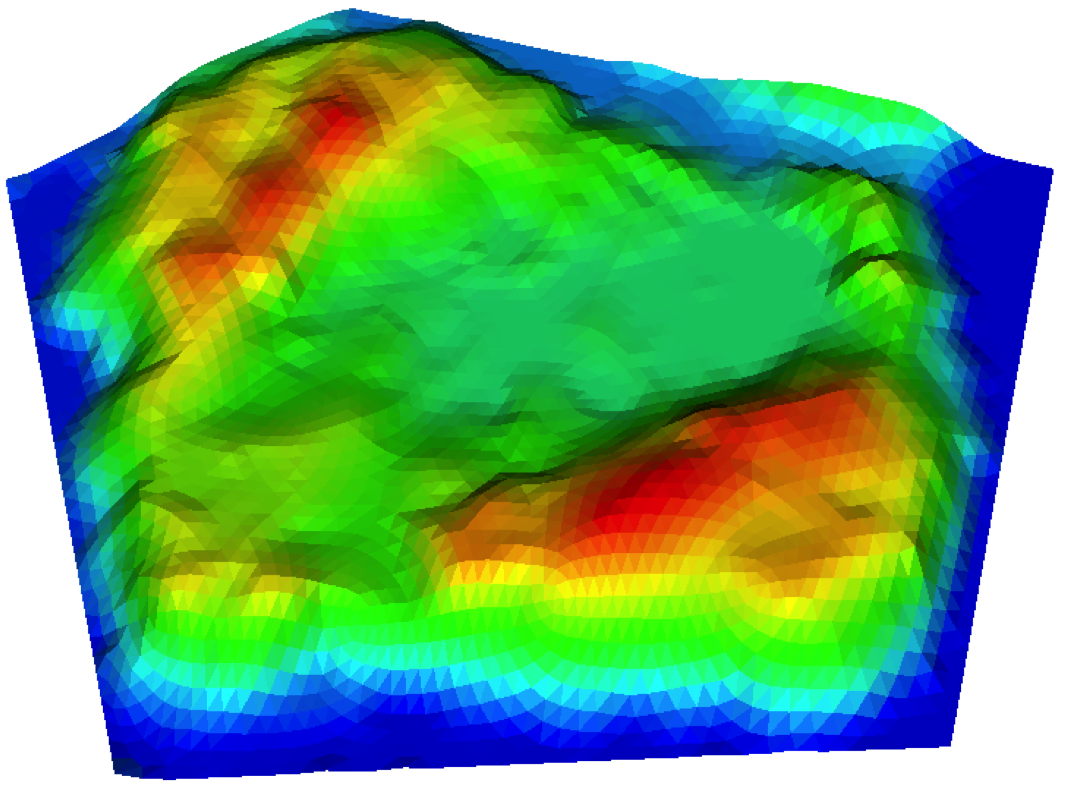
\includegraphics[width=11cm, height=6cm]{./figures/polygons-finescale/3Dpolygon40.png}
%\caption{Microtopograpy for an example ice-wedge polygon from the Barrow Environmental Observatory (BEO).}
%\label{3Dpolygon40}
%\end{figure}

%\begin{figure}
%\centering
%\caption{Volumetric depth versus ponded depth for polygon shown in Figure~\ref{3Dpolygon40}.}
%\label{polygon40}
%\end{figure}

\begin{figure}
\centering
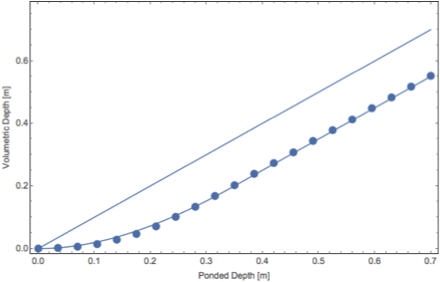
\includegraphics[width=6cm, height=6cm]{./figures/polygons-finescale/picture2.png}
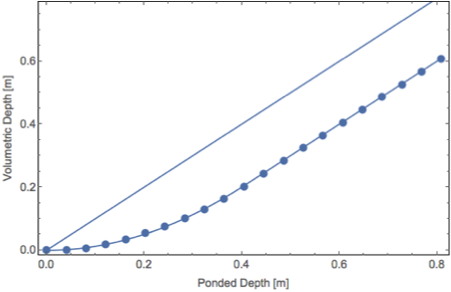
\includegraphics[width=6cm, height=6cm]{./figures/polygons-finescale/picture3.png}\\
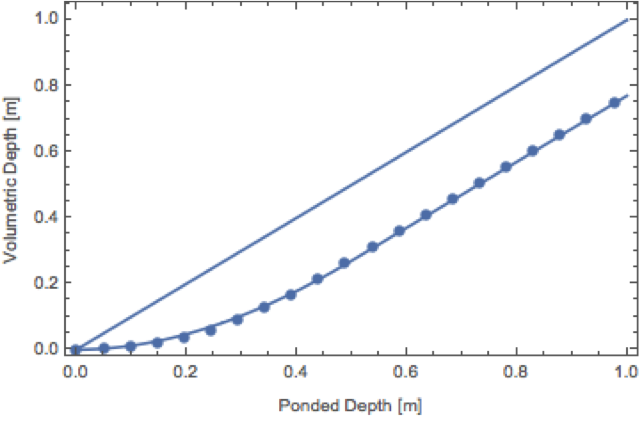
\includegraphics[width=6cm, height=6cm]{./figures/polygons-finescale/polygon40.png}
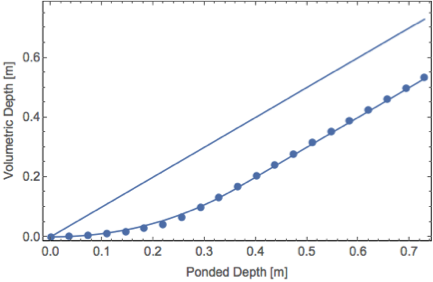
\includegraphics[width=6cm, height=6cm]{./figures/polygons-finescale/picture4.png}
%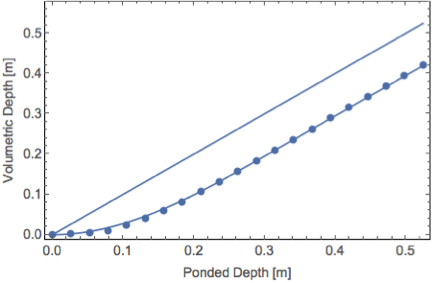
\includegraphics[width=6cm, height=6cm]{./figures/polygons-finescale/picture5.png}
\caption{Volumetric depth versus ponded depth for four ice-wedge polygons. The ice-wedge polygons are displayed in Figure~\ref{IWP-finescale}.}
\label{volumetric-depth-fig1}
\end{figure}

To calculate $\delta_\text{d}$ from the microtopography, we now propose an approach based on site percolation. Specifically, we fill the lowest elevation surface cells until the cluster of inundated cells spans the IWP. This is the percolation threshold. The water height at the percolation threshold defines the $\delta_\text{d}$. Figure~\ref{perc-cluster-poly40} shows the spanning cluster at the percolation threshold for the IWP C40 shown in Figure~\ref{IWP-finescale}. The depression depth calculated this way is 4.1 cm for this IWP.
It is reasonable to assume that the fractional conductance is well approximated by the fractional cross section available to flow, which can be estimated as the ratio of volumetric depth to ponded depth.
\begin{equation}
\Theta {(\delta_\text{d})} \approx \alpha \frac{( \Phi (\delta) - \Phi (\delta_\text{d}))} {\delta} H \left( \delta - \delta_\text{d}\right )
\end{equation}
Where $H$ is the Heaviside function and $\alpha \in (0,1]$ is a drag factor to account for any additional resistance for flow~\cite{panday2004fully}. The numerator is the flowing cross sectional area. Note the velocity is multiplied by ponded depth to get a flux, so the flux appearing in the conservation equations becomes
\begin{equation}
 \delta U = - \alpha ( \Phi (\delta) - \Phi (\delta_\text{d})) H \left( \delta - \delta_\text{d}\right ) \frac{(\delta - \delta_\text{d})^{2/3}}{n_\text{man} (\| \nabla Z \| +\epsilon)^{1/2}} \nabla(Z + \delta)
\end{equation}
\begin{figure}
\centering
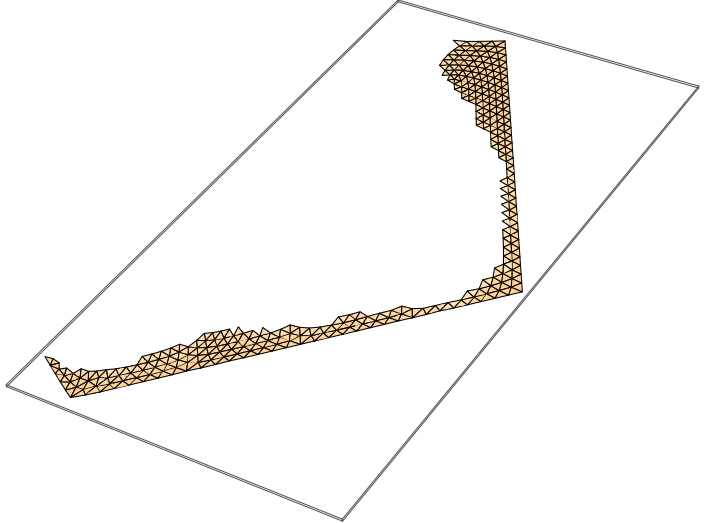
\includegraphics[width=12cm, height=6cm]{./figures/polygons-finescale/percolation-cluster-poly40.png}
\caption{The spanning cluster at the percolation threshold for the IWP C40 (Figure~\ref{IWP-finescale}). The water depth relative to the low point of the microtopography at the percolation threshold defines the depression depth.}
\label{perc-cluster-poly40}
\end{figure}
In summary, we hypothesize that the microtopographic effects on surface flow can be captured with a simple approximation with three parameters that can be computed from the microtopography:

\begin{itemize}
\item Subgrid relief $\delta_\text{max} = Z_{*,\text{max}} -   Z_{*,\text{min}}$, where  $Z_{*,\text{max}}$ and  $Z_{*,\text{min}}$ are the maximum and minimum elevation in the microtopography. 
\item Specific excluded volume $\delta_\text{ex}$, the soil volume above the microtopographic low point normalized by IWP area.
\item Depression depth $\delta$, the difference between the maximum and minimum elevation of the cells in the spanning cluster at the percolation threshold.
\end{itemize}
The subgrid releif and specific excluded volume come directly from the microtopography (univariate statistics). The depression depth requires a simple percolation algorithm to identify the spanning cluster at the percolation threshold. 

\section{Integrated Surface/Subsurface Flow : A Mixed-dimensional Approach}
Simulating fully coupled surface/subsurface thermal hydrology at large spatiotemporal scales is a challenging task. We have recently developed a mixed-dimensional modeling approach to make process-rich integrated surface/subsurface simulations tractable at watershed-scale. The approach discretizes subsurface as independent (one-dimensional) columns and indirectly coupled through a two-dimensional surface system. First, an overland thermal hydrology system is solved and then a family of one-dimensional subsurafce columns is solved. Each column in the family represents a fully coupled surface/subsurface system (without lateral flow) with surface energy balance. The approach is computationally advantageous, enables subcycling processes and allows to track thaw-induced subsidence, for more details the reader is referred to~\cite{jan2017}.


\section{The Advanced Terrestrial Simulator (ATS)}\label{ATS}
Here we provide a very brief overview of the ATS for a reference, for more details about the software infrastructure we refer the reader to~\cite{ecoon2016managing, ats-website}. A fully integrated surface/subsurface and snow distribution modeling capability implemented in ATS are available here~\cite{spainter2016integrated, atchley2015}. As discussed earlier, a mixed-dimensional modeling strategy, mainly designed for the simulations of low-relief permafrost-affected regions, has implemented in ATS and reported in~\cite{jan2017}. The ATS is a publically-available massively parallel computer code, an extended version of Amanzi (flow and reactive transport simulator; see~\cite{moulton2012high}), based on process management tool called Arcos. In ATS, a proces kernel (PK) refers to governing mathematical equations representing a particular (or coupled) physical process(es). Further, Multiprocess Coordinators (MPCs) are available to facilitate coupling amoung PKs. The framework allows to dynamically build a complex/coupled hierarchical model structure. The flexible extensibility feature of the Arcos framework allowed to easily implement our subgrid model and couple with the existing PKs.

\section{Numerical Results and Discussions}\label{numerical-tests}
\FloatBarrier

\subsection{Simulations}
To assess the accuracy of numerical results of our subgrid model, we compare our results with fine-scale simulations and no subgrid model (presented in section \ref{surf-flow-system}). For demonstration purpose, the comparison is made for surface-only flow simulations. In our work, the seven ice-wedge polygon for fine-scale simulations are considered from Barrow Environmental Observatory (BEO) and illustrated in Figure~\ref{IWP-finescale}. The ice-wedge polygons named A, B and C correspond to the NGEE Arctic field sites A, B and C (see Figure~\ref{ngee-arctic-fieldsites}), respectively. Those polygons consist of low-centered, high-centered, with well established troughs (relatively uniform elevation across the trough) and obstructions in the troughs, and hence represent a broader class of polygonal landscape. Table~\ref{subgrid-para} displays subgrid parameters (that is, maximum elevation, specific excluded volume and depression depths) extracted from fine-scale topography of seven IWPs depicted in Figure~\ref{IWP-finescale}.
\begin{center}
\begin{table}[htbp]
\caption{Parameters extracted from fine-scale microtopography for subgrid model. Top row corresponds to different polygons, and first column are the extracted parameters.}\label{subgrid-para}
\begin{tabular}{| c |c|c|c|c|c|c|c|}
\hline
& C06 & C31 & C40 & C44 & C45 & A0 & B01 \\ \hline
 $\delta_\text{max}(m)$ & 0.404 & 0.262 & 0.483 & 0.364 & 0.350 & 0.361 & 0.411 \\ \hline
$\delta_\text{ex}(m)$ & 0.2 & 0.105 & 0.23 & 0.2 & 0.15 & 0.185 & 0.26\\ \hline
$ \delta_\text{d}(m)$ & 0.069 & 0.128 & 0.043 & 0.187 & 0.164 & 0.222 & 0.143 \\ \hline
\end{tabular}

\end{table}
\end{center}

To validate the accuracy of the subgrid model, three sets of numerical experiments are performed and compared with the results of both the fine-scale model and no subgrid model:


\begin{description}\itemsep0pt \parskip0pt
\item [Study I:] Evaluate the subgrid model with (uncalibrated) parameters computed directly from surface microtopography and a fixed drag coefficient (i.e., $\alpha =1$);
\item [Study II:] Evaluate the subgrid model with calibrated depression depth and a fixed drag coefficient (i.e., $\alpha =1$);
\item [Study III:] Evaluate the subgrid model with calibrated depression depth and varying drag coefficient.
\end{description}

Study II is motivated by fine-scale simulations, higher depression depth may delay breakthrough, and would lead to more accumulation of water in the depressions. That said, in Study II we adjust the value the depression depth computed by the percolation algorithm to provide a better fit to the fine-scale results. The process of adjusting model's parameters to replicate the benchmark (e.g., fine-scale computational or real experiments) results is known as calibration. Moreover, higher pressure in the subgrid model affects the overland conductivity and hence the discharge rate. To mimic the behavior of the fine-scale at the time of breakthrough and recession period, the surface roughness is increased to resist flow by lowering the value of drag coefficient.

A pulse numerical test (injection followed by recession) is performed in the above mentioned three numerical studies. That is, we start with a fully dry surface, and inject water at a constant rate at the inlet boundary until breakthrough happens (prescribed flux boundary for a certain period of time), then stop the water supply and let water pass through the outlet (free drainage boundary). The inward and outward arrows shown in Figure~\ref{IWP-finescale} indicate the inlet and outlet boundaries. 
To point out, the entire fine-scale IWP is considered as one coarsened grid cell in the subgrid and no subgrid model -- the elevation of faces depends on the elevation of the corners of the fine-scale IWP.  It is important to mention that the higher (inlet) and lower (outlet) boundaries are chosen based on the average elevation of the faces in the coarsened grid. For instance, the inlet$_2$ in the coarsened grid of the polygon A01 (shown in Figure~\ref{IWP-finescale}) is higher than the outlet$_2$, however, the fine-scale shows inlet$_2$ is lower than outlet$_2$. 

\begin{figure}[!h]
\centering
\vskip -1cm
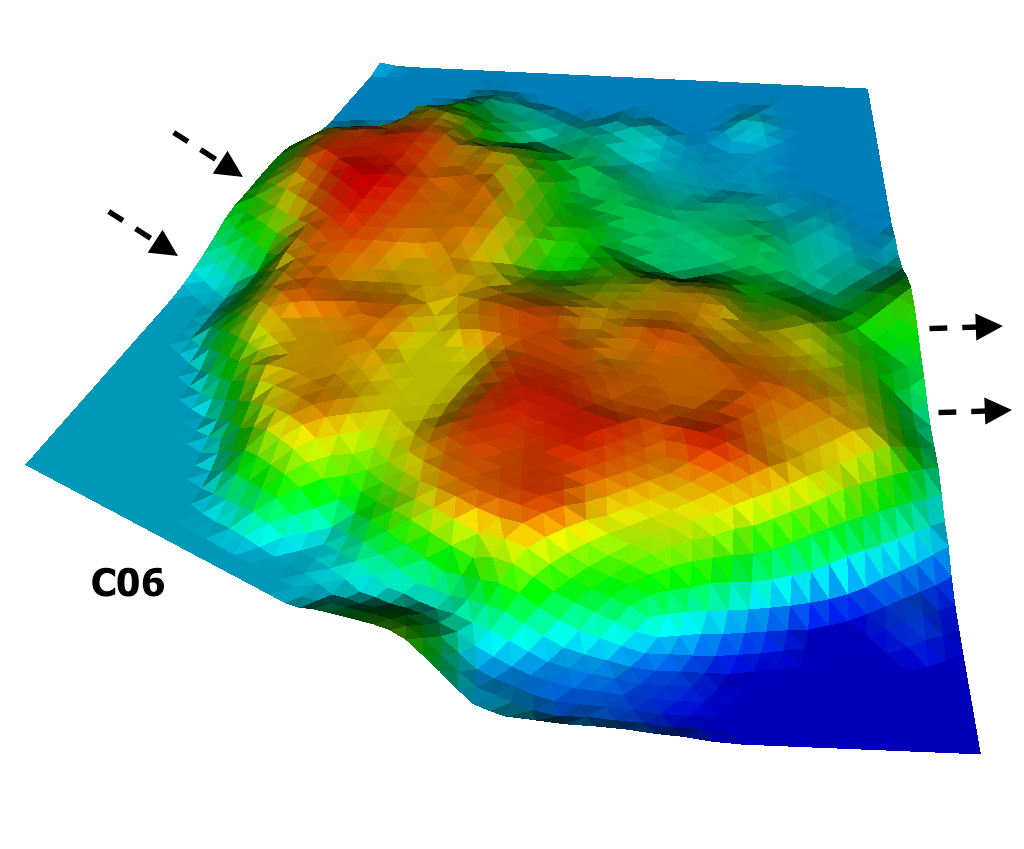
\includegraphics[width=6.2cm, height=4.5cm]{./figures/polygons-finescale/3Dpolygon06-3B.png}
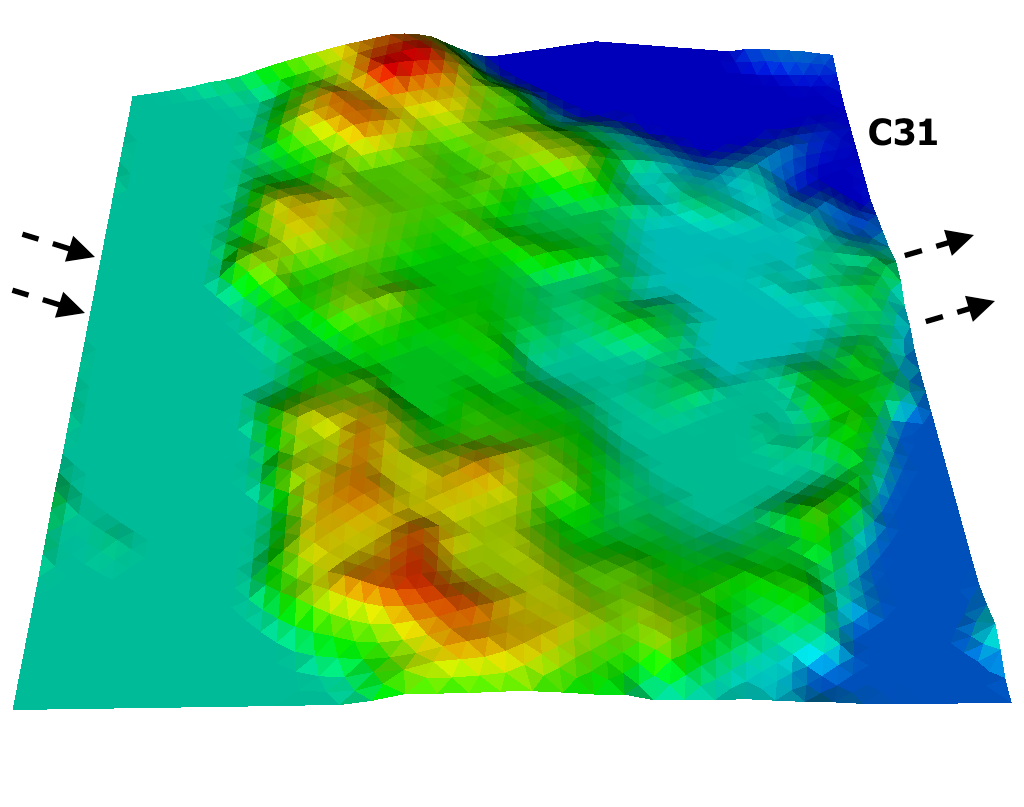
\includegraphics[width=6.2cm, height=4.5cm]{./figures/polygons-finescale/3Dpolygon31-3B.png}\\
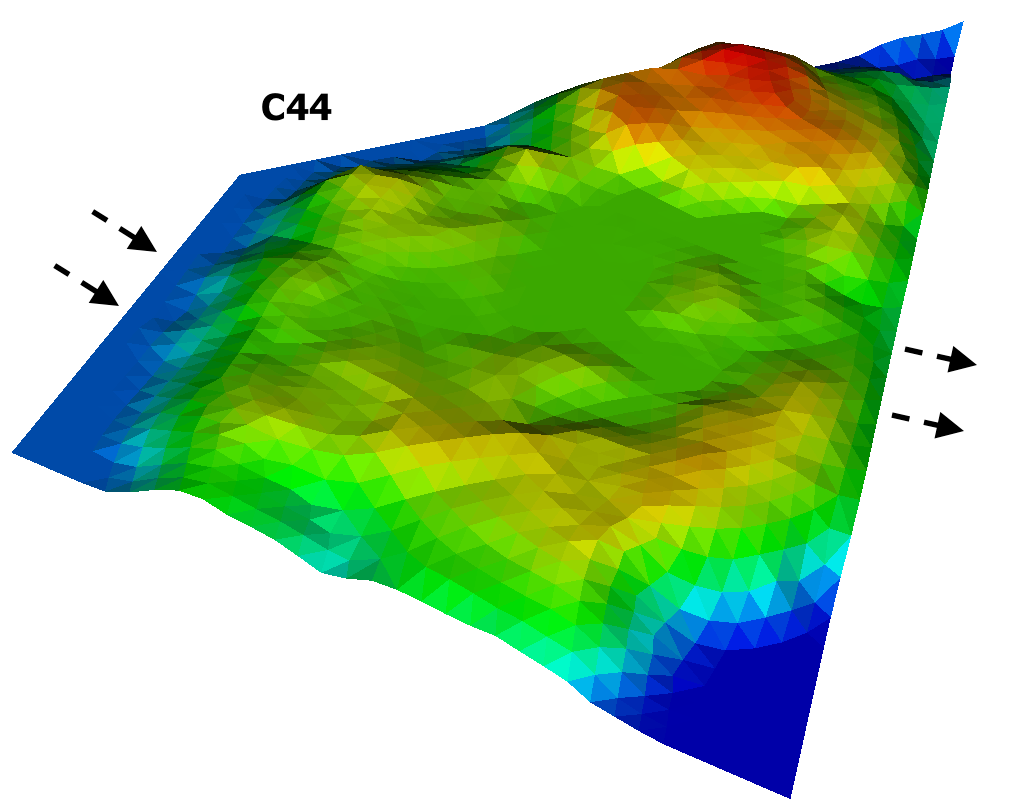
\includegraphics[width=6.cm, height=4.5cm]{./figures/polygons-finescale/3Dpolygon44-3B.png}
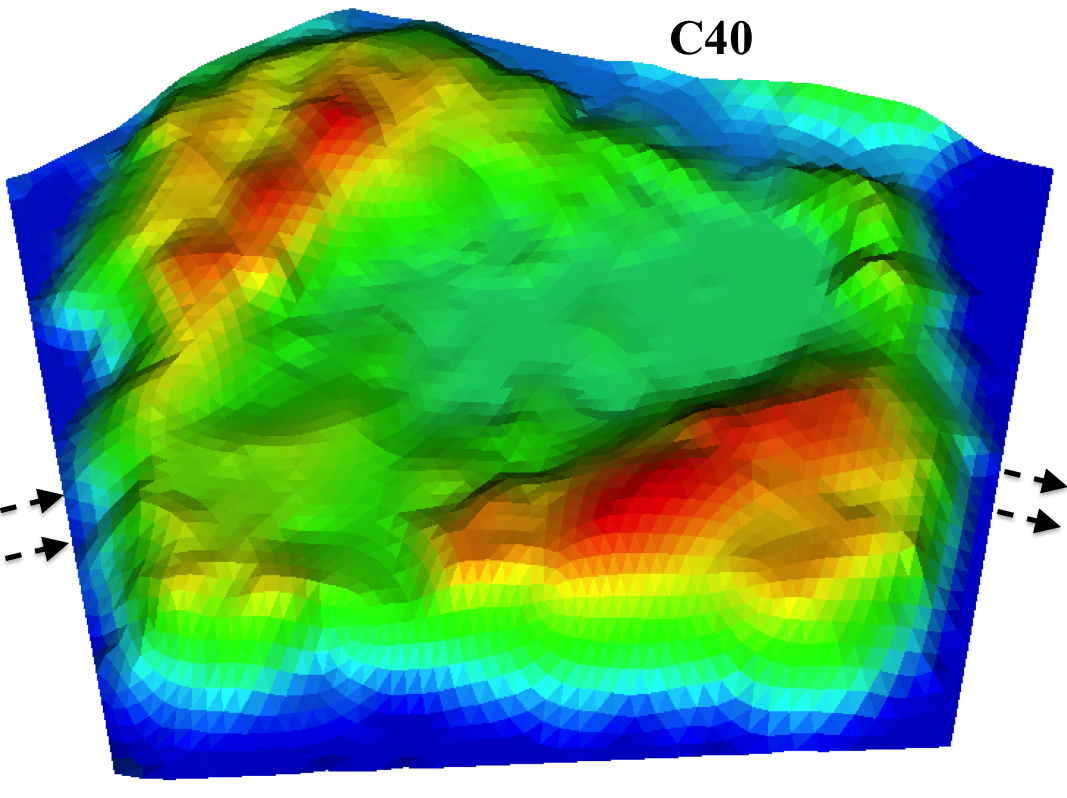
\includegraphics[width=6.2cm, height=4.5cm]{./figures/polygons-finescale/3Dpolygon40-1.png} \\
 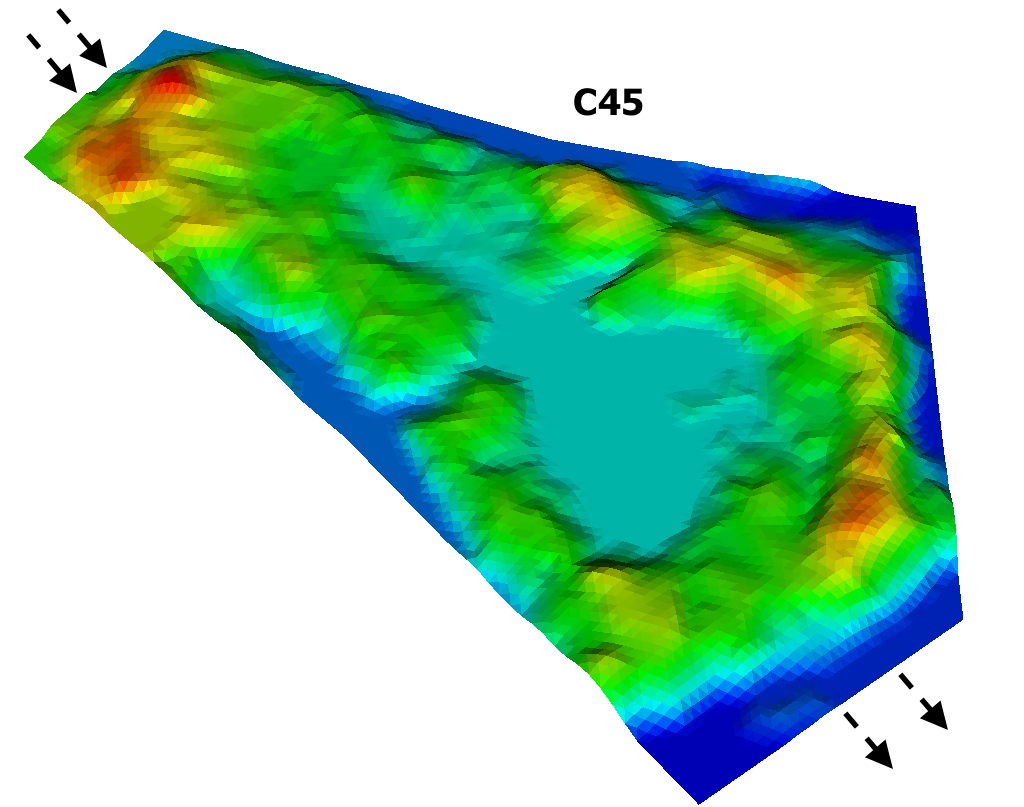
\includegraphics[width=6.2cm, height=4.5cm]{./figures/polygons-finescale/3Dpolygon45-3B.png}
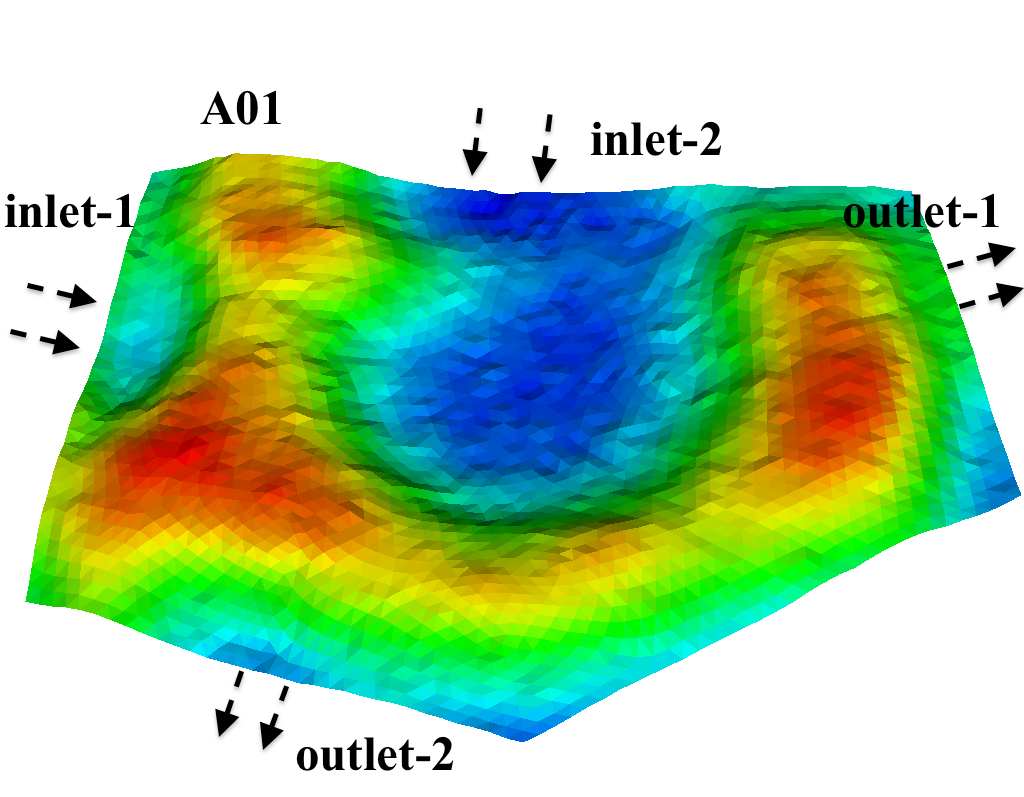
\includegraphics[width=6.2cm, height=4.5cm]{./figures/polygons-finescale/3DpolygonA01-3D.png}\\
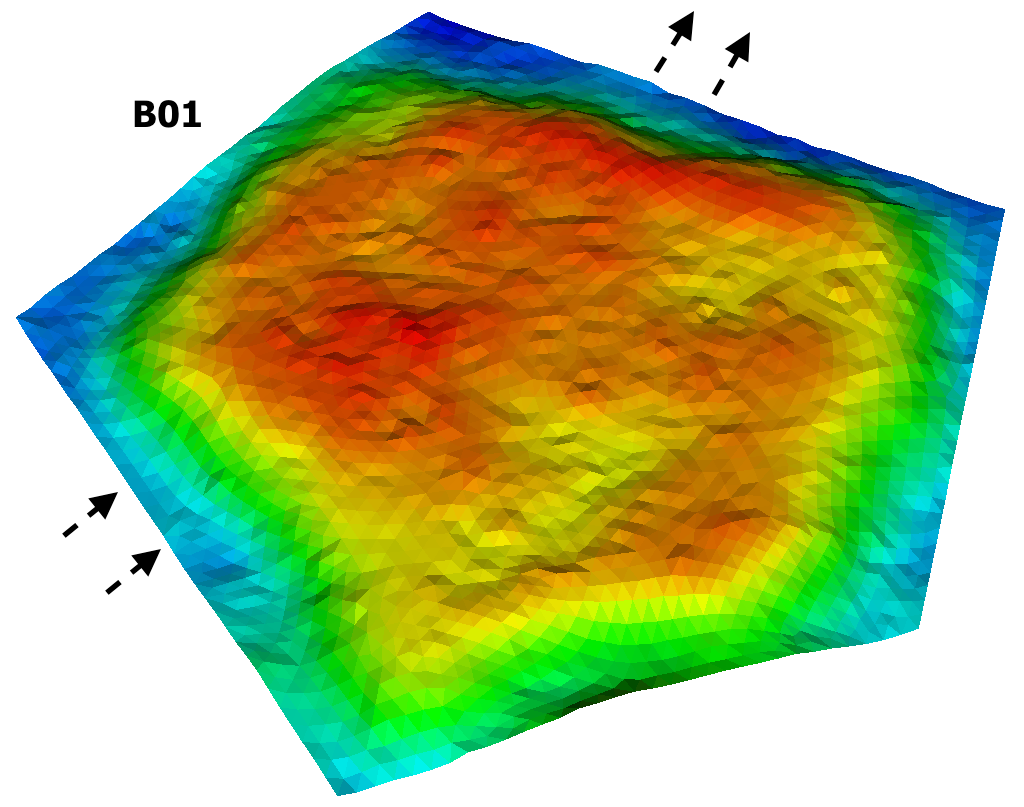
\includegraphics[width=6.2cm, height=4.5cm]{./figures/polygons-finescale/3DpolygonB01-3B.png}
\caption{An Illustration of the microtopography of ice-wedge polygons from Barrow Environmental Observatory (BEO). Red and dark blue spots correspond to high- and low-elevated regions. The arrows indicate inlet and outlet boundaries.}
\label{IWP-finescale}
\end{figure}

The rainfall events are not considered in Studies I, II and III. The presence of a fixed depression depth parameter in the flow law of our subgrid model will not completely allow to replicate the shape of the hydrograph because the fine-scale simulations will show immediate breakthrough. To capture such a behavior it would be more practical to determine the value of the depression depth dynamicly -- change the depression depth as the ponded depth changes. This sort of research will be reported somewhere else. However, in integrated watershed-scale simulations we rain on the surface during the summer, and since in the Arctic regions the rain events are not intense, so we assume the subgrid model should be able to capture accurate surface flow. 


\FloatBarrier
\subsection{Results and Discussions : Single Ice-Wedge Polygons}

Numerical results presented in this subsection correspond to the three studies mentioned above. We compare our results with fine-scale simulations of single IWPs, and we do not present any results on a cluster of fine-scale IWPs. We have carried out detailed simulations on all the polygons shown in Figure~\ref{IWP-finescale}, however, we discuss the results of polygon C44 in more detail and these results serve as a representative of all the remaining polygons as far as the accuracy and shape of the hydrographs are concerned. Figure~\ref{polygon-C44} compares numerical results of the subgrid model with the fine-scale simulations, and no subgrid model of polygon C44. Clearly, Study I fails to match the fine-scale simulations, delayed breakthrough (by 5 hours) in the subgrid model is an indication of higher depression depth computed by the percolation algorithm; see Figure~\ref{polygon-C44}(a). Simulations with a calibrated depression depth, Study II, dramatically improve the shape of the hydrogragh and the water content in the system as shown in see Figure~\ref{polygon-C44}(b). However, a mismatch appears at the time of breakthrough and the beginning of recession period even with the use of a calibrated depression depth. As alluded to earlier, this is due to the huge head gradient between the center and seepage face, and physically makes sense. Figure~\ref{polygon-C44}(c) illustrates the results of Study III, it is evident that our subgrid model reproduces the fine-scale behavior, and the numerical results are identical to the fine-scale simulations. However, a complete mismatch is observed in numerical results of the no subgrid model. Early breakthrough and drier surface at the end of simulation are associated with no obstructions and depressions presence in the no subgrid model. In contrast to the fine-scale and subgrid models, as long as the head gradient is sufficient enough the drainage continues at the outlet.

\begin{figure}
\centering
(a) \hskip -.1cm  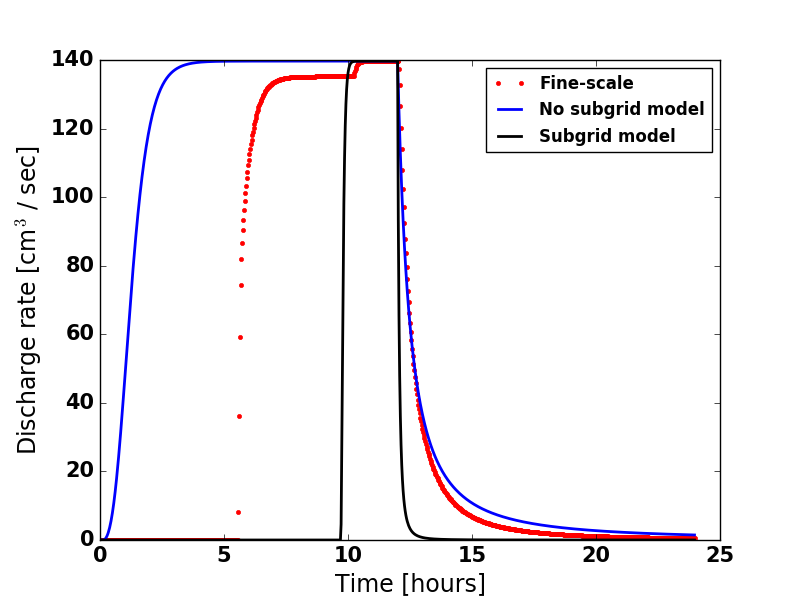
\includegraphics[width=6.cm, height=5.2cm]{./figures/POLYGON44/POLYGON44discharge.png}
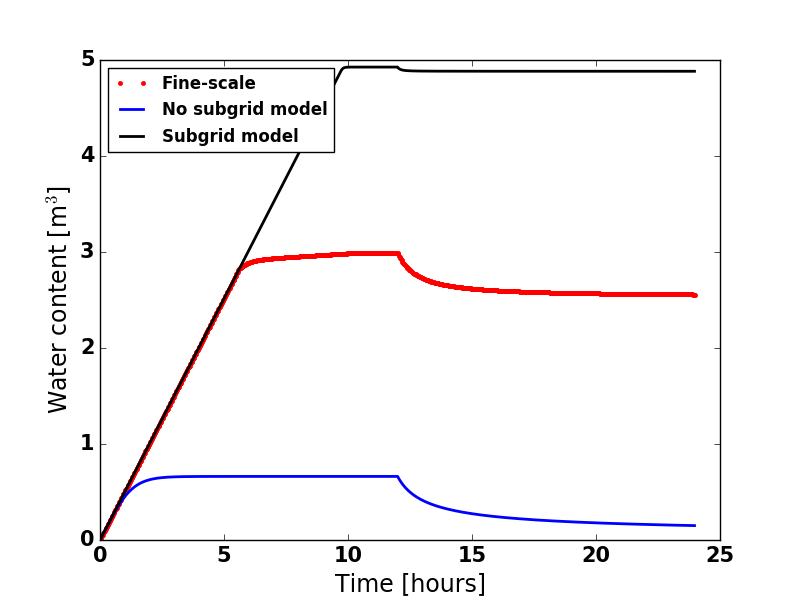
\includegraphics[width=6.cm, height=5.2cm]{./figures/POLYGON44/POLYGON44watercontent.png}\\
(b) \hskip -.1cm 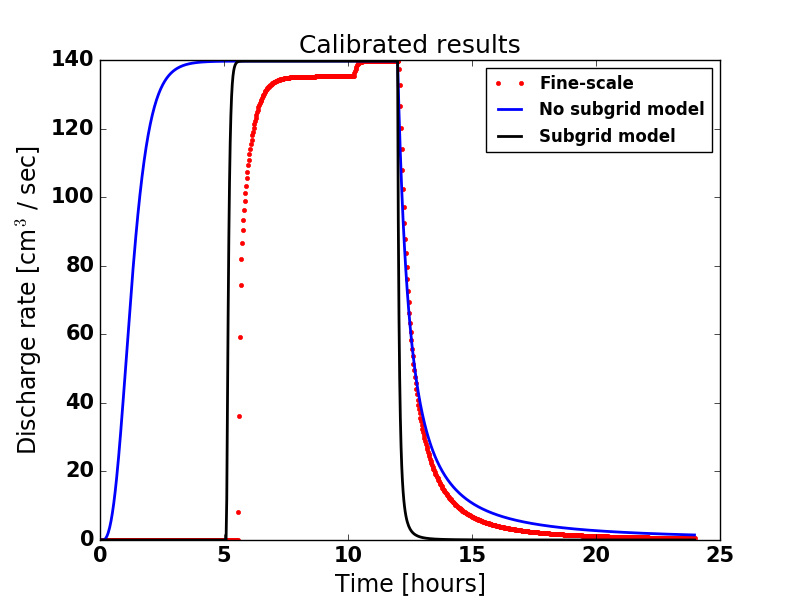
\includegraphics[width=6.cm, height=5.2cm]{./figures/POLYGON44/POLYGON44dischargeCalibDD.png}
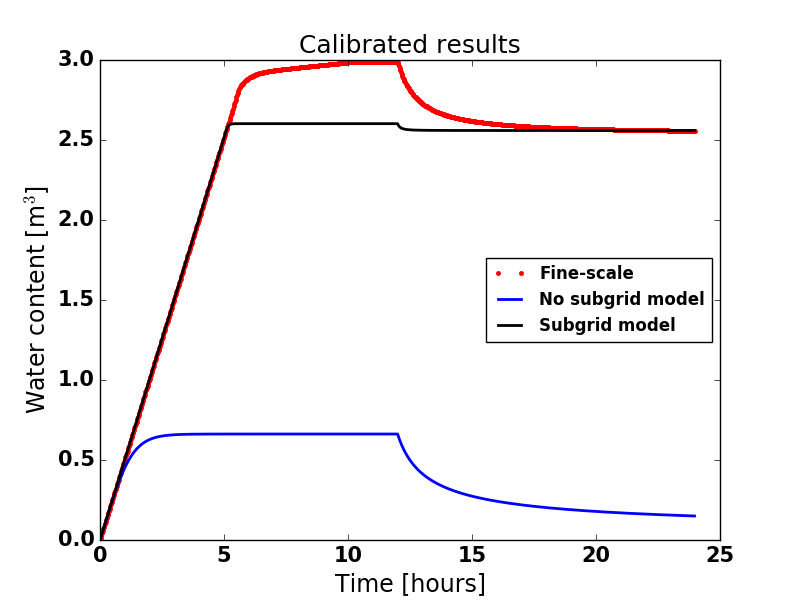
\includegraphics[width=6.cm, height=5.2cm]{./figures/POLYGON44/POLYGON44watercontentCalibDD.png} \\
(c) \hskip -.1cm 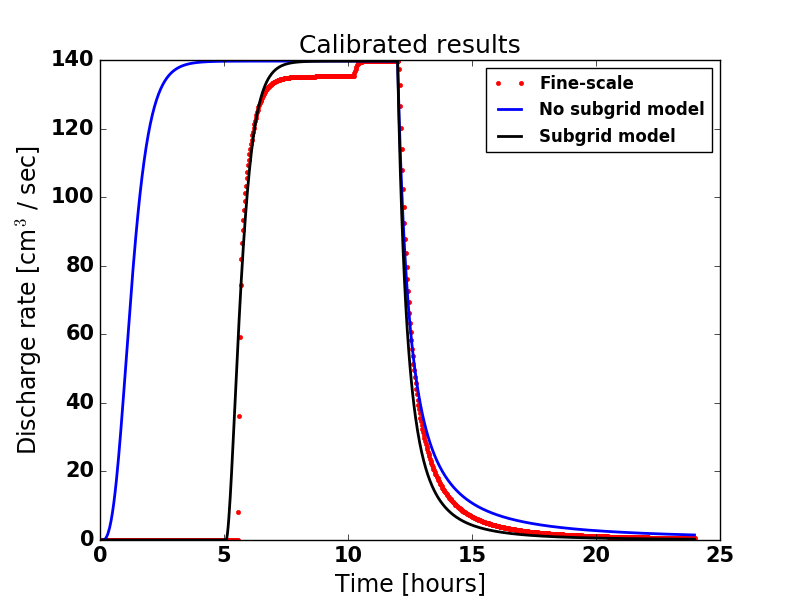
\includegraphics[width=6.cm, height=5.2cm]{./figures/POLYGON44/POLYGON44dischargeCalibDDManning.png}
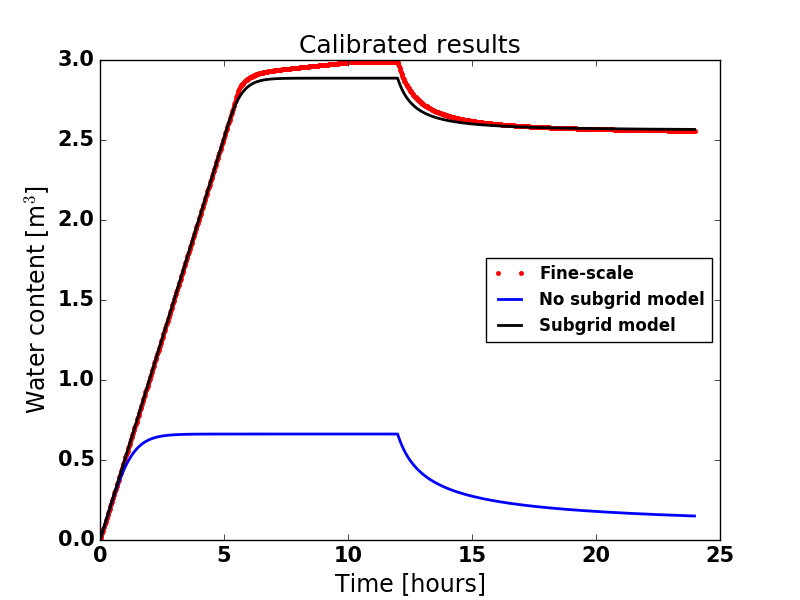
\includegraphics[width=6.cm, height=5.2cm]{./figures/POLYGON44/POLYGON44watercontentCalibDDManning.png}
\caption{(Polygon C44) Comparison of the numerical results of the subgrid model with the fine-scale and no subgrid model results. Rows (top to bottom) correspond to Study I, II and III, respectively.}
\label{polygon-C44}
\end{figure}

Figure~\ref{polygon-C06} compares the numerical results of Study I and III with the fine-scale and no subgrid model. The percolation algorithm computed the depression depth very accurately for polygon C06, and calibration (Study II) is not required. Similar to the results of polygon C44, the high overland conductivity in the subgrid model is reduced by increasing the surface roughness (i.e., lowering $\alpha$). It improves the results and replicate the recession period of the fine-scale results. Figure~\ref{polygon-C06} also displays the water retained in the subgrid and fine-scale models, the match is very close. 
For polygon C31, the results of the subgrid model are strongly affected by the depression depth in Study I, and lead to a mismatch. However, the results of Study II and III indicate that calibrated values of the depression depth and increased surface roughness improved the simulated results dramatically and yield a close match as depicted in Figure~\ref{polygon-C31}. 
Numerical simulations correspond to polygons C40, C45, A01, and B01 are shown in Figures~\ref{polygon-C40}, \ref{polygon-C45}, \ref{polygon-A01}, and \ref{polygon-B01}, respectively. In Figure~\ref{polygon-A01}, the results correspond to inlet$_2$ and outlet$_2$ boundaries, the results using inlet$_1$ and outlet$_1$ are discussed later in this subsection. Overall, the results of the subgrid model are very encouraging and consistently yield a better fit to the fine-scale results as compared to the no subgrid model. 

\begin{figure}
\centering
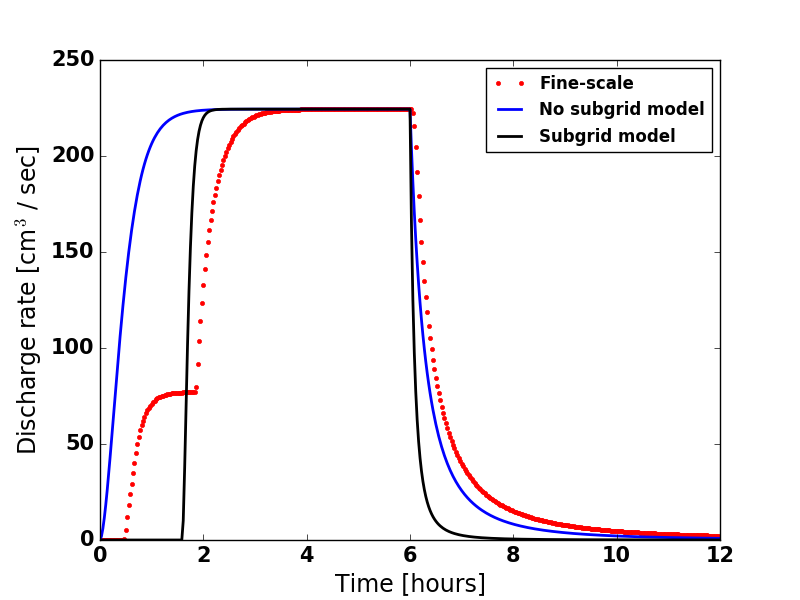
\includegraphics[width=6.2cm, height=6cm]{./figures/POLYGON06/POLYGON06discharge.png}
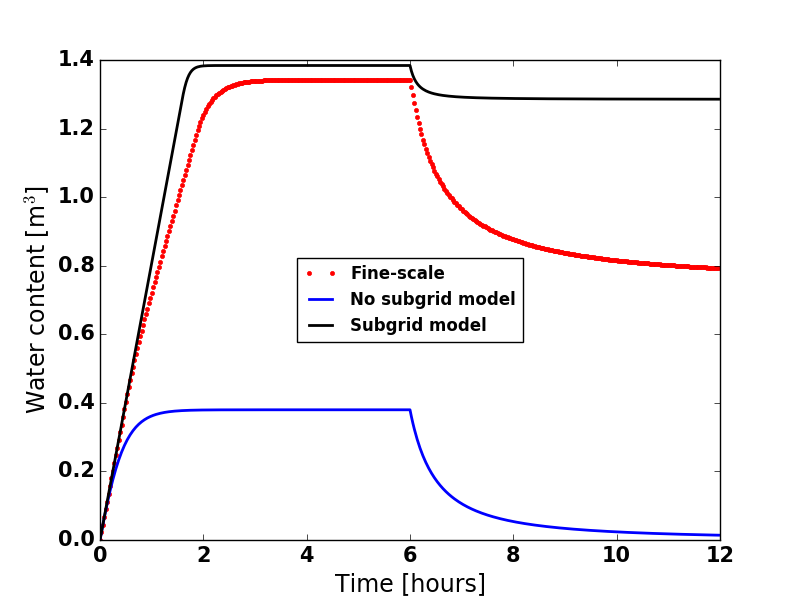
\includegraphics[width=6.2cm, height=6cm]{./figures/POLYGON06/POLYGON06watercontent.png}\\
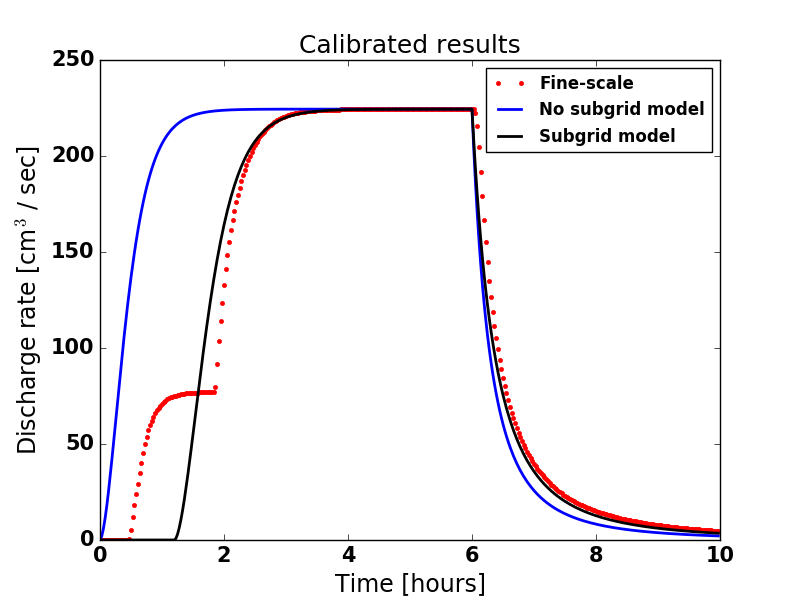
\includegraphics[width=6.2cm, height=6cm]{./figures/POLYGON06/POLYGON06dischargeCalibDDManning.png}
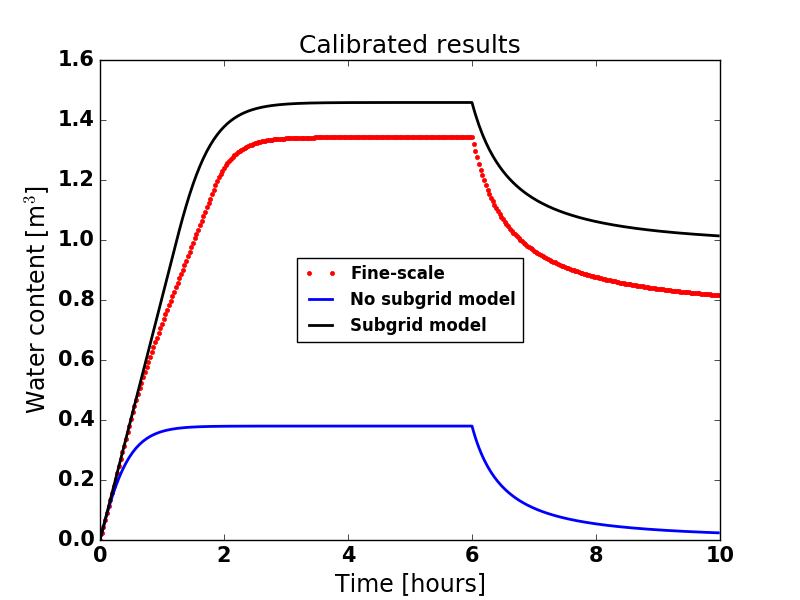
\includegraphics[width=6.2cm, height=6cm]{./figures/POLYGON06/POLYGON06watercontentCalibDDManning.png}
\caption{(Polygon C06) Comparison of the numerical results of the subgrid model with the fine-scale and without subgrid model results. Top and bottom row correspond to Study I and Study III, respectively.}
\label{polygon-C06}
\end{figure}


\begin{figure}
\centering
%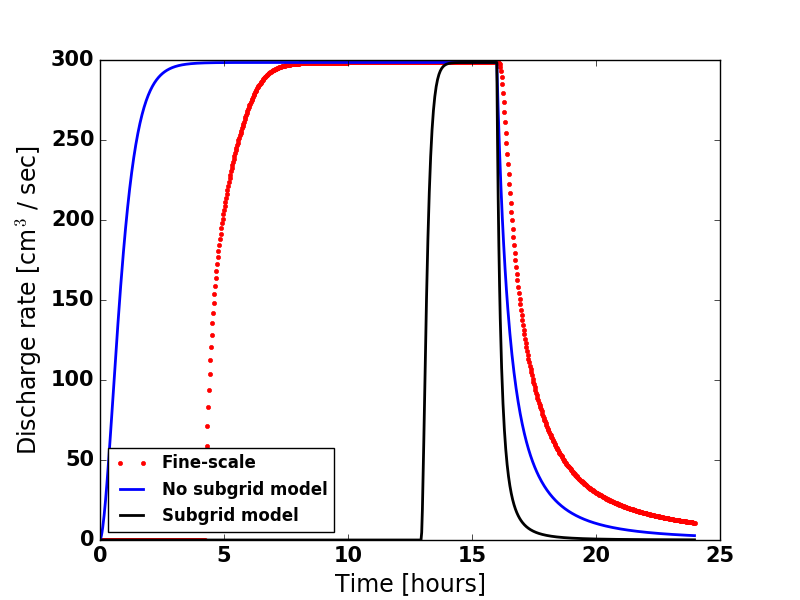
\includegraphics[width=6.2cm, height=5cm]{./figures/POLYGON31/POLYGON31discharge.png}
%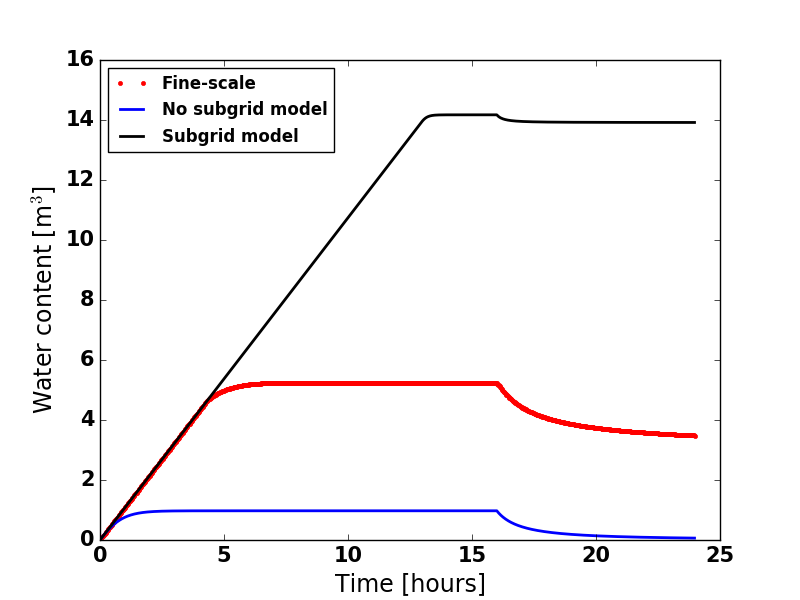
\includegraphics[width=6.2cm, height=5cm]{./figures/POLYGON31/POLYGON31watercontent.png}\\
%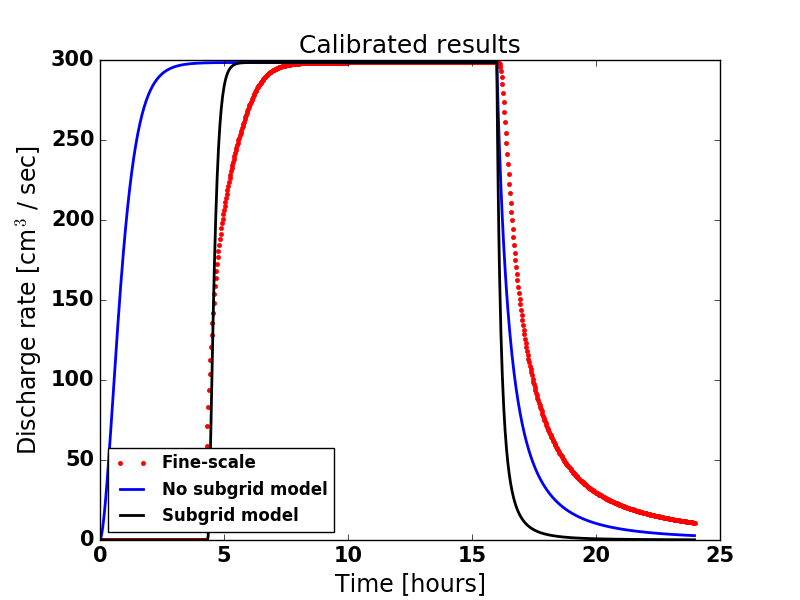
\includegraphics[width=6.2cm, height=5cm]{./figures/POLYGON31/POLYGON31dischargeCalibDD.png}
%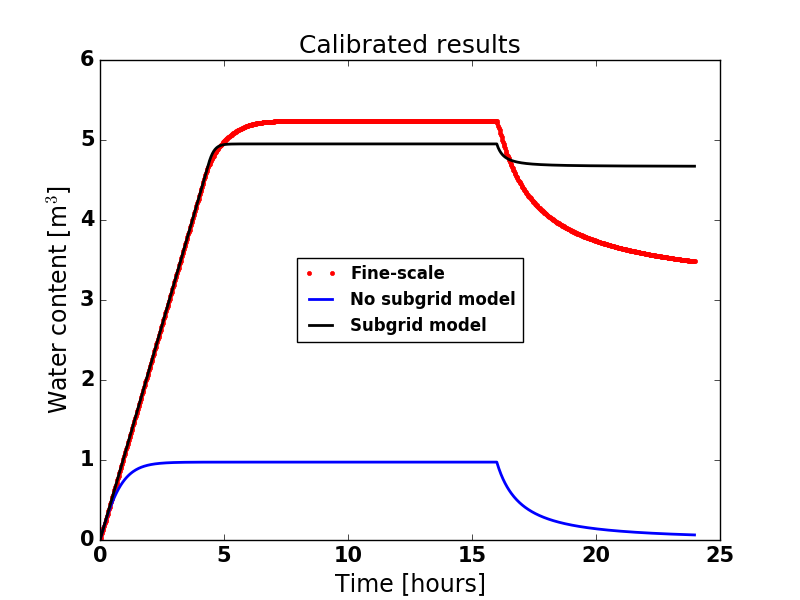
\includegraphics[width=6.2cm, height=5cm]{./figures/POLYGON31/POLYGON31watercontentCalibDD.png} \\
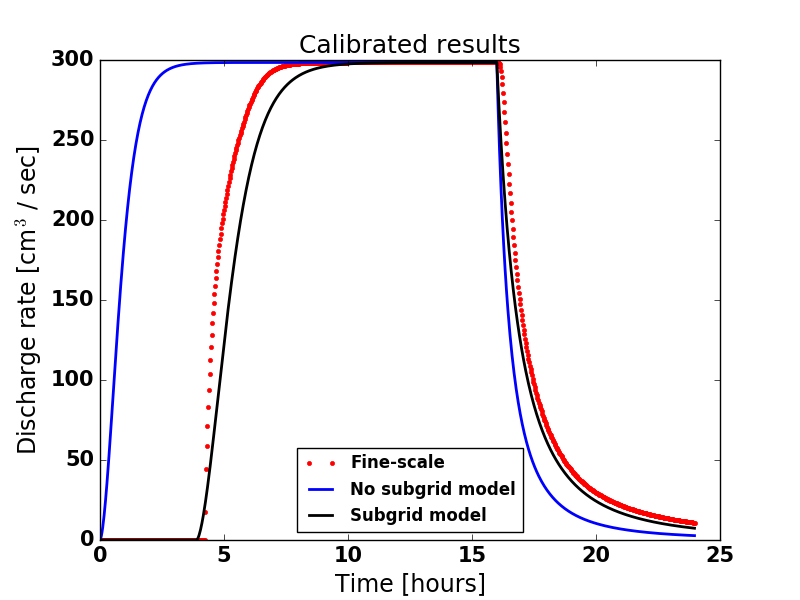
\includegraphics[width=6.2cm, height=5cm]{./figures/POLYGON31/POLYGON31dischargeCalibDDManning.png}
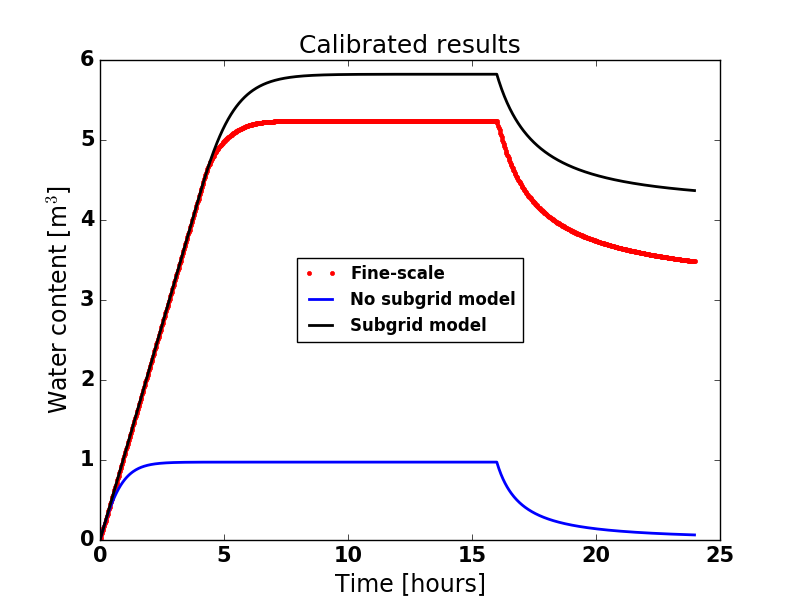
\includegraphics[width=6.2cm, height=5cm]{./figures/POLYGON31/POLYGON31watercontentCalibDDManning.png}
\caption{(Polygon C31) Comparison of the numerical results of the subgrid model with the fine-scale and no subgrid model. Results corresponded to Study III.}
\label{polygon-C31}
\end{figure}


\begin{figure}
\centering
%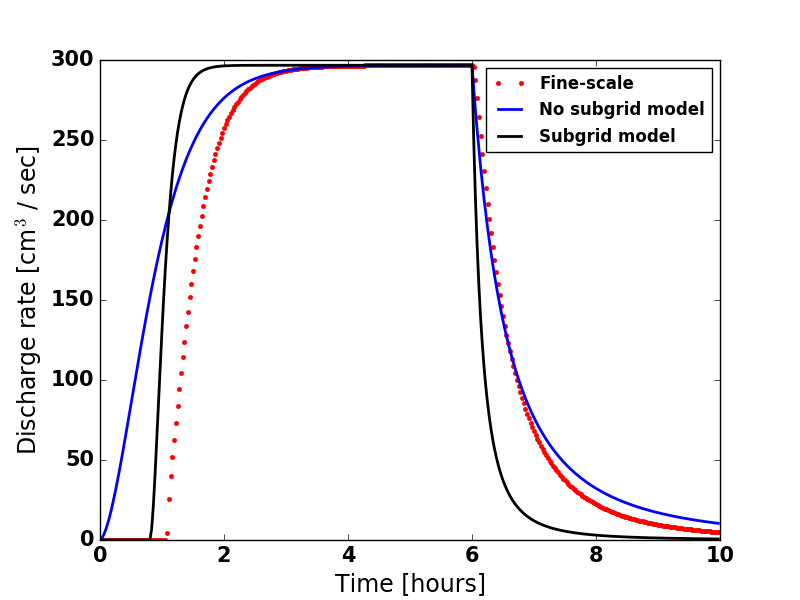
\includegraphics[width=6.2cm, height=5.5cm]{./figures/POLYGON40/POLYGON40discharge.png}
%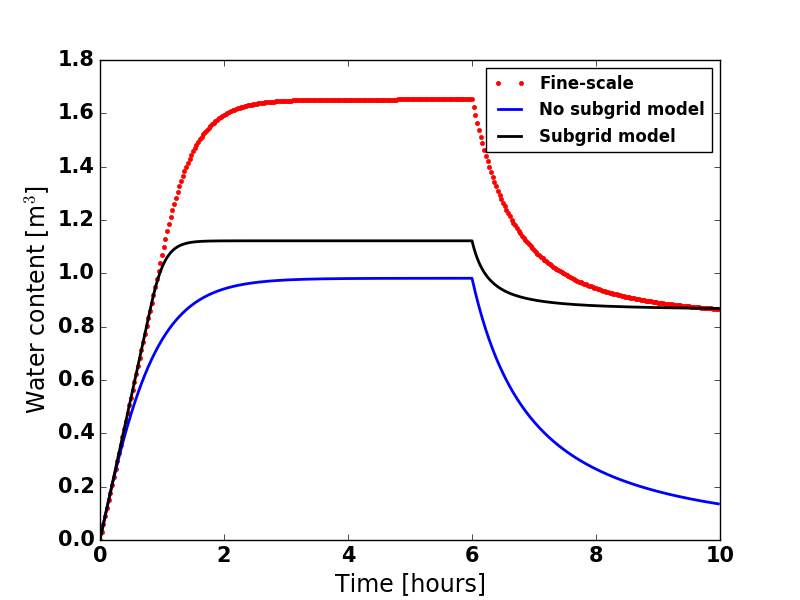
\includegraphics[width=6.2cm, height=5.5cm]{./figures/POLYGON40/POLYGON40watercontent.png}\\
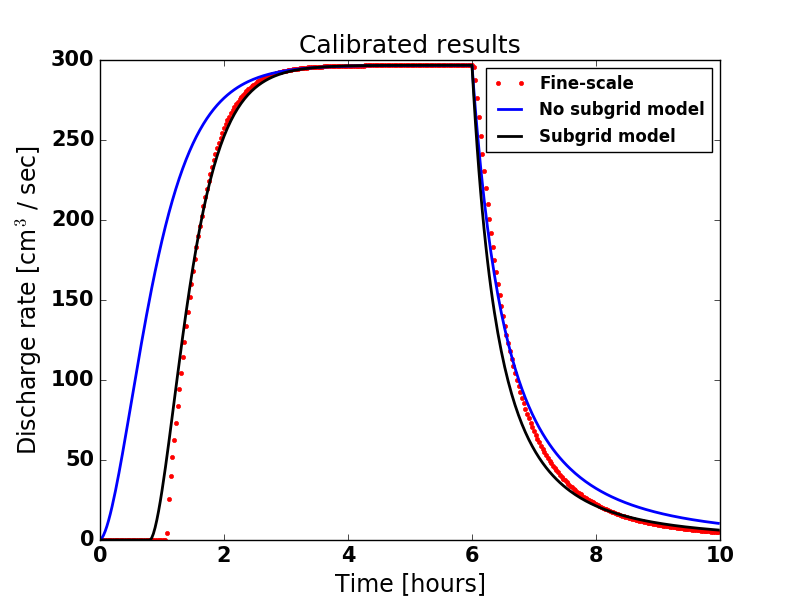
\includegraphics[width=6.2cm, height=5.5cm]{./figures/POLYGON40/POLYGON40dischargeCalibManning.png}
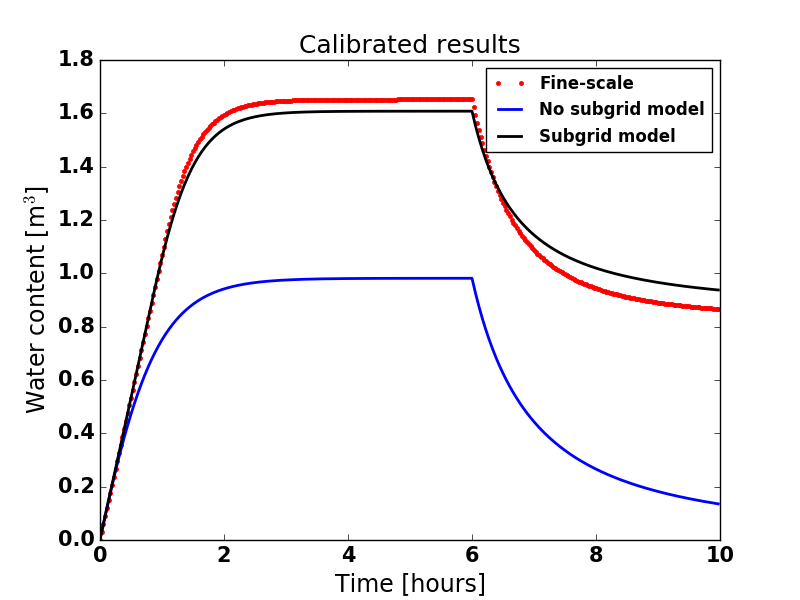
\includegraphics[width=6.2cm, height=5.5cm]{./figures/POLYGON40/POLYGON40watercontentCalibManning.png}
\caption{(Polygon C40) Comparison of the numerical results of the subgrid model with the fine-scale and without subgrid model results.}
\label{polygon-C40}
\end{figure}




\begin{figure}[!h]
\centering
%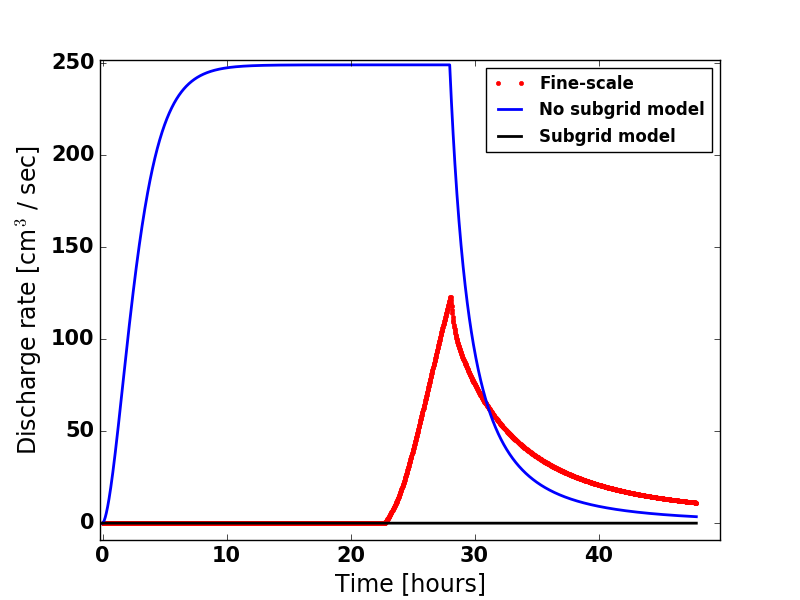
\includegraphics[width=6.2cm, height=5.5cm]{./figures/POLYGON45/POLYGON45discharge2.png}
%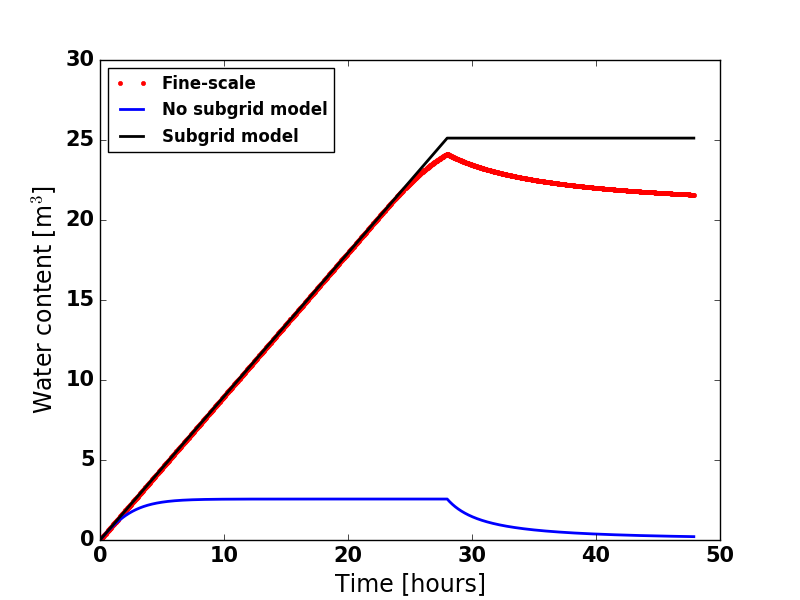
\includegraphics[width=6.2cm, height=5.5cm]{./figures/POLYGON45/POLYGON45watercontent.png}\\
%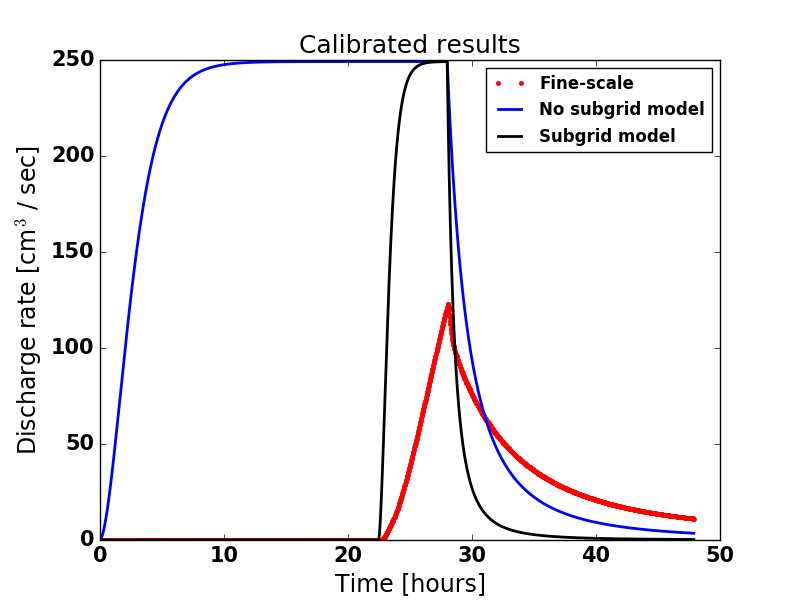
\includegraphics[width=6.2cm, height=5.5cm]{./figures/POLYGON45/POLYGON45dischargeCalibDD.png}
%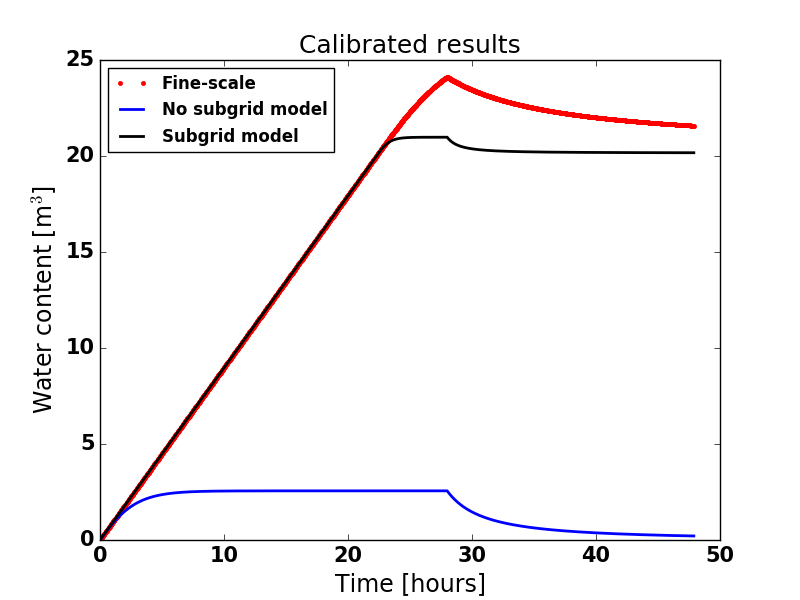
\includegraphics[width=6.2cm, height=5.5cm]{./figures/POLYGON45/POLYGON45watercontentCalibDD.png} \\
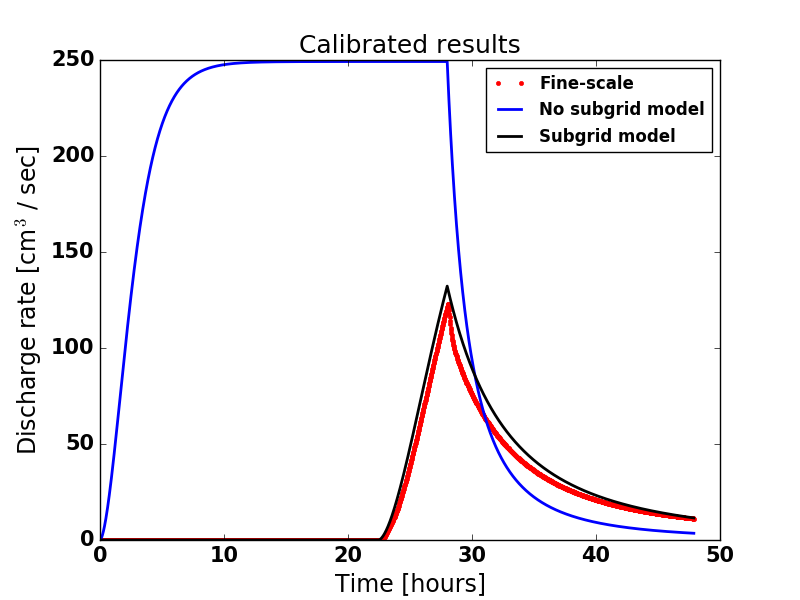
\includegraphics[width=6.2cm, height=5.5cm]{./figures/POLYGON45/POLYGON45dischargeCalibDDManning.png}
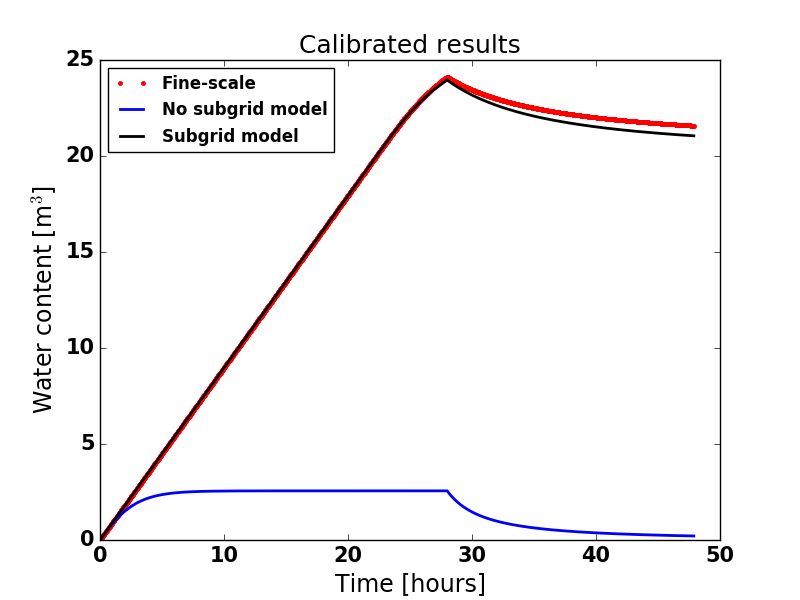
\includegraphics[width=6.2cm, height=5.5cm]{./figures/POLYGON45/POLYGON45watercontentCalibDDManning.png}
\caption{(Polygon C45) An illustration of the numerical results of the subgrid model, the fine-scale and no subgrid model. Simulations correspond to Study III.}
\label{polygon-C45}
\end{figure}




\begin{figure}[!h]
\centering
%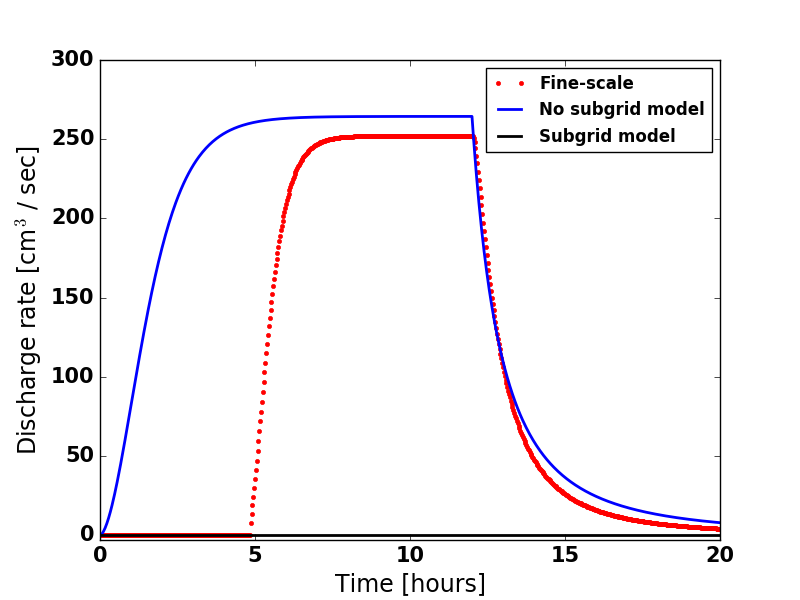
\includegraphics[width=6.2cm, height=5.5cm]{./figures/POLYGON_A01/POLYGON_A01discharge.png}
%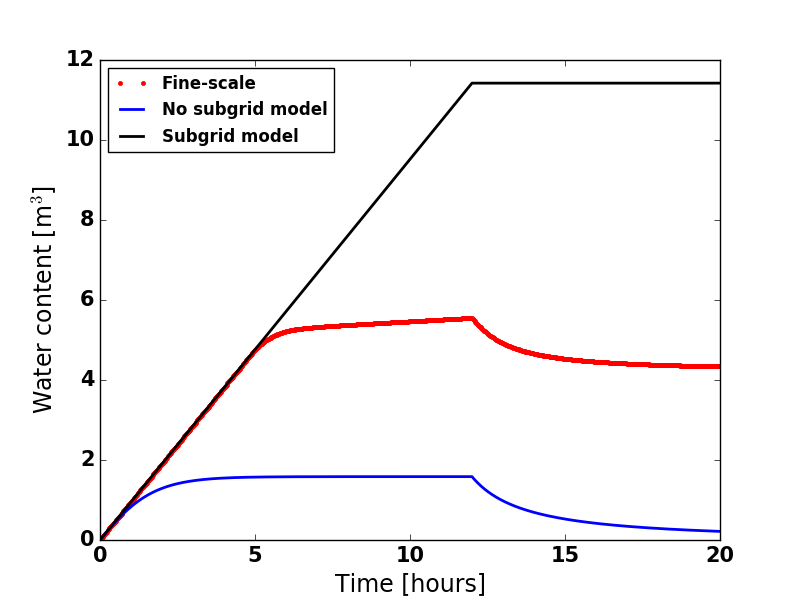
\includegraphics[width=6.2cm, height=5.5cm]{./figures/POLYGON_A01/POLYGON_A01watercontent.png}\\
%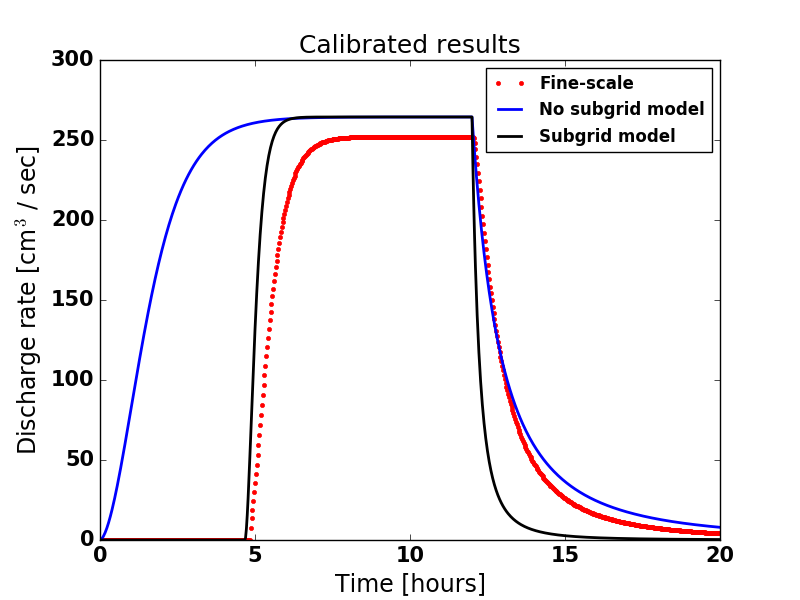
\includegraphics[width=6.2cm, height=5.5cm]{./figures/POLYGON_A01/POLYGON_A01dischargeCalibDD.png}
%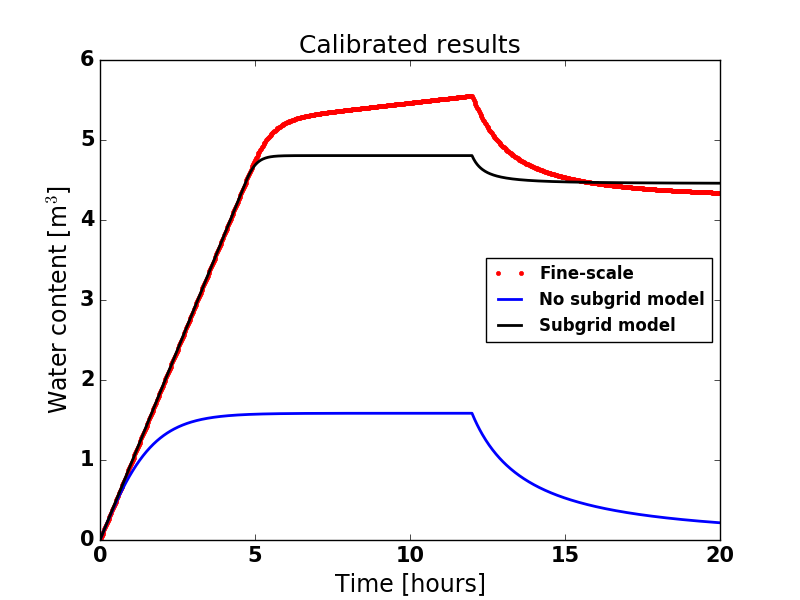
\includegraphics[width=6.2cm, height=5.5cm]{./figures/POLYGON_A01/POLYGON_A01watercontentCalibDD.png} \\
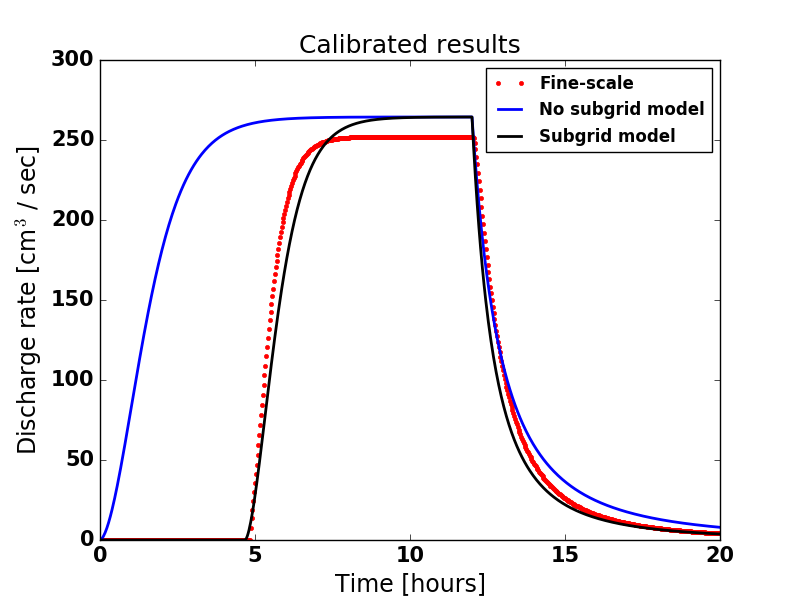
\includegraphics[width=6.2cm, height=5.5cm]{./figures/POLYGON_A01/POLYGON_A01dischargeCalibDDManning.png}
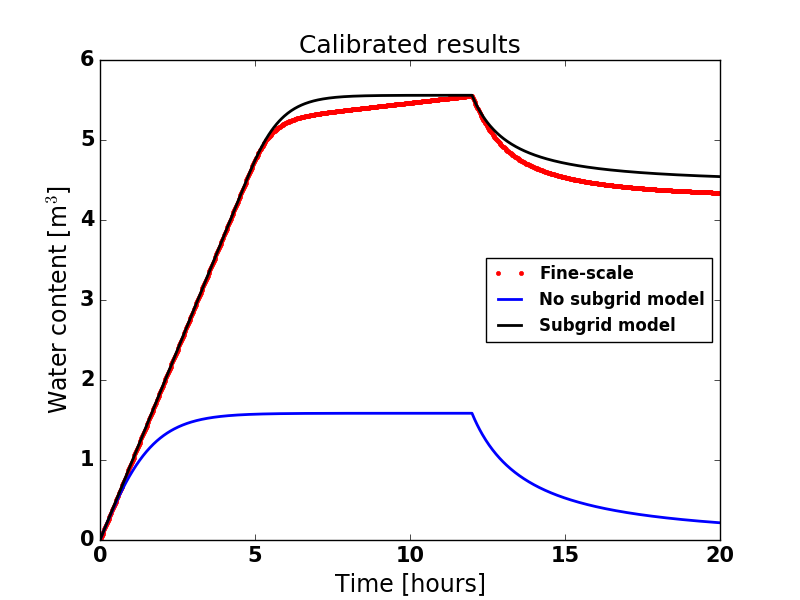
\includegraphics[width=6.2cm, height=5.5cm]{./figures/POLYGON_A01/POLYGON_A01watercontentCalibDDManning.png}
\caption{(Polygon A01) Comparison of the hydrographs and water content from the numerical simulation of the fine-scale, subgrid and no subgrid models. Results correspond to  inlet$_2$ and outlet$_2$ boundaries.}
\label{polygon-A01}
\end{figure}

\begin{figure}[!h]
\centering
%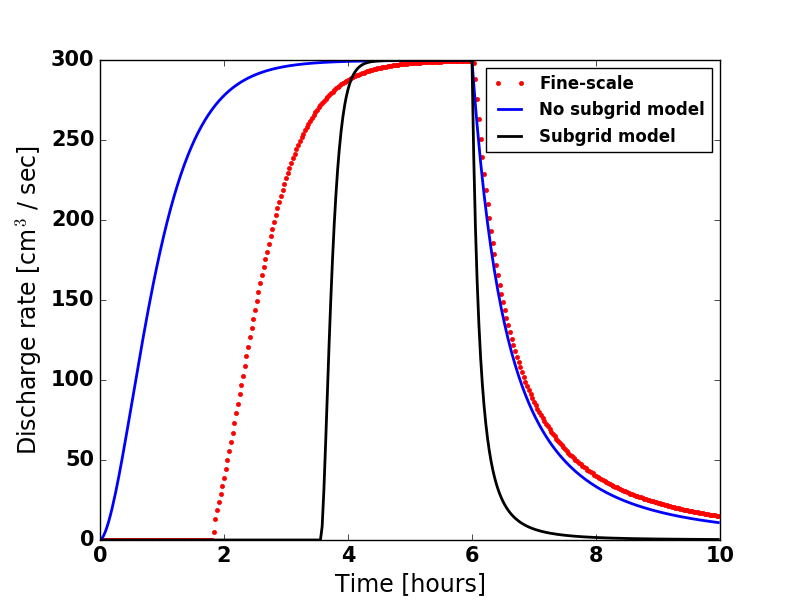
\includegraphics[width=6.2cm, height=5.5cm]{./figures/POLYGON_B01/POLYGON_B01discharge.png}
%\includegraphics[width=6.2cm, height=5.5cm]{./figures/POLYGON_B01/POLYGON_B01watercontent.png}\\
%\includegraphics[width=6.2cm, height=5.5cm]{./figures/POLYGON_B01/POLYGON_B01dischargeCalibDD.png}
%\includegraphics[width=6.2cm, height=5.5cm]{./figures/POLYGON_B01/POLYGON_B01watercontentCalibDD.png} \\
\includegraphics[width=6.2cm, height=5.5cm]{./figures/POLYGON_B01/POLYGON_B01dischargeCalibDDManning.png}
\includegraphics[width=6.2cm, height=5.5cm]{./figures/POLYGON_B01/POLYGON_B01watercontentCalibDDManning.png}
\caption{(Polygon B01) Comparison of the numerical results of the subgrid model with the fine-scale and without subgrid model results.}
\label{polygon-B01}
\end{figure}

\subsection{Results and Discussions : Watershed-scale Integrated Surface/Subsurface}
To assess the importance of microtopographic effects on the watershed-scale hydrology, three different scenarios based on the depression and obstruction features of polygons are developed; (S$_1$) topography at a scale of polygons does not vary, that is, each polygon has same features, (S$_2$) uniformly generated spatially varying topography, (S$_3$) normally generated spatial heterogeneity in the topography.  
We demonstrate that independent of the choice of the polygonal landscape, the subgrid model and hence the fine-scale microtopography has significant effects on the watershed-scale hydrology. Fig.~\ref{hetero-sg-parameters} plots the depression depths of polygonal tundras described in S$_2$ and S$_3$. Other subgrid parameters (maximum elevation and excluded volume) also vary spatially but are not shown here, however the drag factor $\alpha$ is set to $0.16$ across the domain. Table~\ref{dist-limits} displays extreme values of the subgrid parameters of the three hypothetical polygonal tundras. The excluded soil volume is made correlated to the maximum ponded depth, this correlation can be seen for real ice-wedge polygons as well, see Table~\ref{subgrid-para}. 

For model spin-up and boundary conditions the reader is referred to~\cite{spainter2016integrated}, and the soil (moss, peat, mineral)  properties are consistent with the work reported in~\cite{atchley2015}. After spinup, the model was forced over a 10-year loop with daily meteorological data from 2013 at Barrow, Alaska. Numerical results presented in this subsection correspond to the tenth year. Discharge rate and cumulative discharge from the watershed for the no subgrid model and the subgrid model for three landscapes are compared in Fig.~\ref{mdm-discharge}. Clearly, higher peak and more cumulative discharge in the no subgrid model as compared to the subgrid model are evident, and a consequence of ignored processes associated with depressions and obstructions. Fig.~\ref{volumetric-pd} shows volumetric ponded depth of the subgrid and no subgrid models. Since the depressions pond water and yield less cumulative discharge, so more surface wetness is observed in the subgrid model. The ponded water in the surface depressions is solely available for infiltration and evaporation. Average gas saturation resulted from no subgrid and subgrid models are plotted in Fig~\ref{gas-saturation}, decrease in the gas saturation in the subgrid model implies more infiltration. Average gas saturation is computed as follows:
\begin{equation}
S_g^{\text{avg}} = \frac{1}{m}\sum\limits_{i=1}^{m}{ \left ( \sum\limits_{j=1}^{n} S_g(i,j) \right) }.
\end{equation}
Here $m$ denotes total number of subsurface columns and $n$ represents total number of cells per column.
To conclude, numerical simulations of the integrated surface/subsurface model with subgrid parameterization show significant influences on the surface wetness and hydrographs, however relatively less effects on the active layer thickness and thermal surface/subsurface conditions for the current climate.
Note that in this work, we are not making an attempt to compare simulated results of the subgrid model for different polygonal tundras. For watershed-scale integrated simulations, the focus is on the comparison of the numerical results of the subgrid and no subgrid models.
\begin{figure}[!h]
\centering
\includegraphics[width=6.2cm, height=5.5cm]{./figures/DeprDepth/Mrun1SG.png}
\includegraphics[width=6.2cm, height=5.2cm]{./figures/DeprDepth/Mrun1SG-Hist.png} \\
\includegraphics[width=6.2cm, height=5.5cm]{./figures/DeprDepth/Mrun4SG.png}
\includegraphics[width=6.2cm, height=5.2cm]{./figures/DeprDepth/Mrun4SG-Hist.png} \\
\caption{An illustration of randomly generated landscapes. Uniformly (top) and normally (bottom) distributed depressions.}
\label{hetero-sg-parameters}
\end{figure}

\begin{table}
\caption{Range of subgrid parameters for three hypothetical polygonal tundras. Left column correspond to the type of polygonal tundra.}
\begin{tabular}{|p{9.5mm}|p{7mm}|c|p{7mm}|p{7mm}|c|p{7mm}|c|c|c|c|c|c|p{7mm}c|p{6mm}|c|}
\hline
\multirow{2}{*}{} & \multicolumn{3}{c|}{$\delta_\text{d}(m)$} & \multicolumn{3}{c|}{$\delta_\text{max}(m)$}  & \multicolumn{3}{c|}{$\delta_\text{ex}(m)$}  \\ \hhline{~---------}
& max & min & mean & max & min & mean & max & min & mean \\ \hline
S$_1$ & 0.13 & 0.13 & 0.13 & 0.35 & 0.35 & 0.35 & 0.15 & 0.15 & 0.15 \\
S$_2$ & 0.03 & 0.13 & 0.08 & 0.15 & 0.4 & 0.27 & 0.047 & 0.22 & 0.14 \\
S$_3$ & 0.037 & 0.165 & 0.106 & 0.315 & 0.436 & 0.375 & 0.144 & 0.235 & 0.188 \\ \hline
\end{tabular}
\label{dist-limits}
\end{table}


\begin{figure}[!h]
\centering 
\includegraphics[width=6.2cm, height=5.5cm]{./figures/MDM/DischargeRate-All-10yr.png}
\includegraphics[width=6.2cm, height=5.5cm]{./figures/MDM/CumulativeDischarge-All-10yr.png} 
\caption{Comparing the discharge rate and cumulative discharge resulted from the no subgrid model and the subgrid model for three landscapes (\textcolor{red}{S$_1$}, \textcolor{black}{S$_2$}, and \textcolor{green}{S$_3$}).}
\label{mdm-discharge}
\end{figure}

\begin{figure}[!h]
\centering 
\includegraphics[width=6.2cm, height=5.5cm]{./figures/MDM/VPD-NSG-10yr-165d.png}
\includegraphics[width=6.2cm, height=5.5cm]{./figures/MDM/VPD-Mrun4SG-10yr-165d.png} 
\caption{Volumetric ponded depth of the no subgrid (left) and subgrid (right) models for polygonal tundra S$_2$. Red implies dry surface.}
\label{volumetric-pd}
\end{figure}

\begin{figure}[!h]
\centering 
\includegraphics[width=9.2cm, height=5.5cm]{./figures/MDM/GS-Mrun1SG-10yr.png}
\caption{Shown is the average gas saturation from the simulations of the no subgrid model and subgrid model for polygonal tundra S$_2$. Average is obtained by summing the gas saturation of a column and then averaging over all the columns.}
\label{gas-saturation}
\end{figure}

\subsection{Additional Remarks}
{
\itemize{

\item Not surprisingly, the subgrid model favors high surface roughness that swings the results toward fine-scale simulations. A high agreement between the results of the subgrid model and fine-scale simulations due to reduced runoff is an indication of a needed drag coefficient in the flow law. A linear regression fit to the drag factor vs. the depression depth is depicted in Figure~\ref{curvefit-dd-manning}. The drag factor varies between zero and one, as the depression depth decreases the drag factor goes to unity -- a representation of flow law over a flat surface. The fit indicates the resistance to flow increases with increasing depression. This finding is highly consistent with the discussion regarding the conductance terms in~\cite{panday2004fully}.

\item An empirical relation correlating the uncalibrated (directly measured from the microtopographic data) and calibrated (insight from fine-scale simulations to adjust the uncalibrated values) depression depths is shown in Figure~\ref{curvefit-dd-manning}. The fitted curve with the coefficient of determination 0.82 yields a good match. As a subject for future research, the application of invaded percolation (flow in the direction of least resistance) algorithm could provide more accurate depression depths, and would probably overcome the issues of calibrating parameters and/or location of inlet and outlet boundaries.

\item For low-centered polygons such as C45 and A01, Study I (uncalibrated results) fails to match the hydrograph of the fine-scale simulations -- no breakthrough happens if uncalibrated depression depths are used. Fine-scale simulations show that low-elevated regions may remain completely dry if they are not located in the main flow channel which is trivial. However, as stated earlier, our percolation algorithm fills the lowest elevation cells until the cluster of inundated cells spans the IWP. Thereby, the direction of the injected fluid is important. For instance, considering polygon A01, the results are not comparable if the inlet and outlet are at sides inlet$_1$ and outlet$_1$, respectively. However, if the inlet and outlet are switched to inlet$_2$ and outlet$_2$ a desirable match is obtained; see Figure~\ref{polygon-A01-fig2}.

\item Most of our numerical experiments show that the subgrid model outperforms the no subgrid model even when the fine-scale flow behavior is not completely captured.

\item When the inlet boundary has obstructions (for example, polygon C06 in Figure~\ref{IWP-finescale}) and divides the incoming water into different flow channels, the water reaches the outlet boundary at different times and lead to a dual-peak (or may be multiple-peak) hydrograph.  Due to only one grid cell in the subgrid model, the dual-peak behavior is not possible to capture.

}
\begin{figure}[!h]
\centering
\includegraphics[width=6.cm, height=5.5cm]{./figures/fittedcurve-dd-1.png}
\includegraphics[width=6.cm, height=5.5cm]{./figures/fittedcurve-manning.png}
\caption{ (Left) Linear fitted-curve to the depression depth data. (Right) Drag factor vs. calibrated depression depth.}
\label{curvefit-dd-manning}
\end{figure}

\begin{figure}[!h]
\centering
(a)\includegraphics[width=6.cm, height=5.5cm]{./figures/POLYGON_A01/POLYGON_A01discharge.png}
\includegraphics[width=6.cm, height=5.5cm]{./figures/POLYGON_A01/POLYGON_A01watercontent.png}\\
(b)\includegraphics[width=6.cm, height=5.5cm]{./figures/POLYGON_A01/POLYGON_A01discharge-CalibDDManningTest3.png}
\includegraphics[width=6.cm, height=5.5cm]{./figures/POLYGON_A01/POLYGON_A01WC-CalibDDManningTest3.png}
%\includegraphics[width=6.2cm, height=5.5cm]{./figures/POLYGON_A01/POLYGON_A01dischargeCalibDDManning.png}
%\includegraphics[width=6.2cm, height=5.5cm]{./figures/POLYGON_A01/POLYGON_A01watercontentCalibDDManning.png}
\caption{(Polygon A01) An illustration of the numerical results based on the choice of the inlet and outlet boundaries. The orientation affects the match between the fine-scale and subgrid model. (a) inlet$_1$ and outlet$_1$ boundary; (b) inlet$_2$ and outlet$_2$  boundary.}
\label{polygon-A01-fig2}
\end{figure}
}

\section{Conclusions}\label{conclusion}

The subgrid model presented in this paper is aimed at incorporating the microtopographic effects in the governing equations for the simulations of integrated surface/subsurface processes at watershed-scale. Standalone fine-scale surface simulations are tractable with the existing sophisticated computing tools. However, a significant challenge is how to capture accurate flow behavior in the watershed-scale integrated models because fine-scale simulations of integrated models at such a scale are not feasible.
Seven fine-scale ice-wedge polygons are considered to demonstrate that the effect of surface microtopography can be captured in coarsened models through the use of a subgrid model. Numerical results of the subgrid model compare very well with the fine-scale simulations. Our analysis shows that accurate estimate of depression depth is a determining factor for a close match between subgrid and fine-scale simulations.
Three different studies are conducted to estimate the parameters for the subgrid representation: (1) direct measurements from topography; (2) insight from fine-scale simulations to calibrate; (3) and empirical adjustment of topography-derived values. 
Thus the effort to obtain a reasonable match with the fine-scale simulations using coarsened meshes with a subgrid representation was highly successful. The model is applied to 468 polygons watershed and a comparison is made with no subgrid model. Our preliminary numerical results demonstrate that the subgrid parameterization significantly effects the surface wetness and shape of hydrographs. However, the subgrid model has relatively less significance in regard to the active layer thickness and thermal surface/subsurface conditions for permafrost-affected regions under the current climate.

The subgrid model's ability to accurately capture fine-scale flow behavior provides confidence that a few parameters extracted from the available microtopographic data can be used to incorporate the fine-scale effects in watershed-scale integrated models.
However, more research is needed to extend the approach developed here to more accurately simulate problems involving both runoff and rain/snow precipitation.


\section*{References}

\bibliography{reference}

\end{document}



